%\fs{whole section probably needs to fit in max 2 pages}

\sys{}'s execution protocol has three goals: 1) to offer clients an interactive transaction interface \fs{too obvious?}, 2) to be scalable, and 3) to maintain independent operability \fs{and Byzantine independence, Serializability}.

\sys{} achieves these goals by combining optimistic client-side execution with an aggressive, but Byzantine resilient, concurrency control (CC) scheme that maintains Byz-Serializability. 
\iffalse
 \la{We seem to have already made this points in the intro tio the section} \changebars{}{\sys leaves clients responsible for executing the transactions they submit, and allows every client, in parallel, to execute arbitrary interactive transactions using read RPC's, instead of submitting stored procedured that must be ordered and executed by replica servers.}  
 \fi By relying on optimistic rather than pessimistic CC schemes such as 2-phase-locking (2PL), \sys{} forgoes costly coordination to acquire locks, and sidesteps the concern of Byzantine clients refusing to relinquish locks.

\iffalse
\la{I would just remove the following} 
\changebars{}{Before we detail Indicus’s transaction processing and validation mechanism, we first discuss the CC that Indicus imple- ments as the latter are functions of the precise CC requirements.}
\fi

\subsection{\sys{}'s Concurrency Control}

%%% Explain MVTSO itself only briefly. Then explain how we make it for for byz
% 1) bound timestamps, 2) make writes visible late only, 3) only allow f+1 matchin uncommitted writes, 4) read timestamps
%Afterwards: explain execution interface. After that explain validation check. Then have overarching example
\iffalse
% we need to change a few things:
0) timestmap bound
1) Read validity
2) deferred writes
3) read uncommitted
4) byz read timestamps (read lock implies you had access control, at that point it is no different than issuing a tx and completing. But we do not want to give the power to abort for no reason. It should be traceable.
\fi

\fs{fig doesnt make so much sense before reading the whole thing} \fs{cut this preamble?}
Figure \ref{fig:MVTSOEX} shows an example trace of \sys operational behaviors under different request processing orders (assume $f=1$) that we use to guide the remaining outline.

\begin{figure*}
\begin{center}
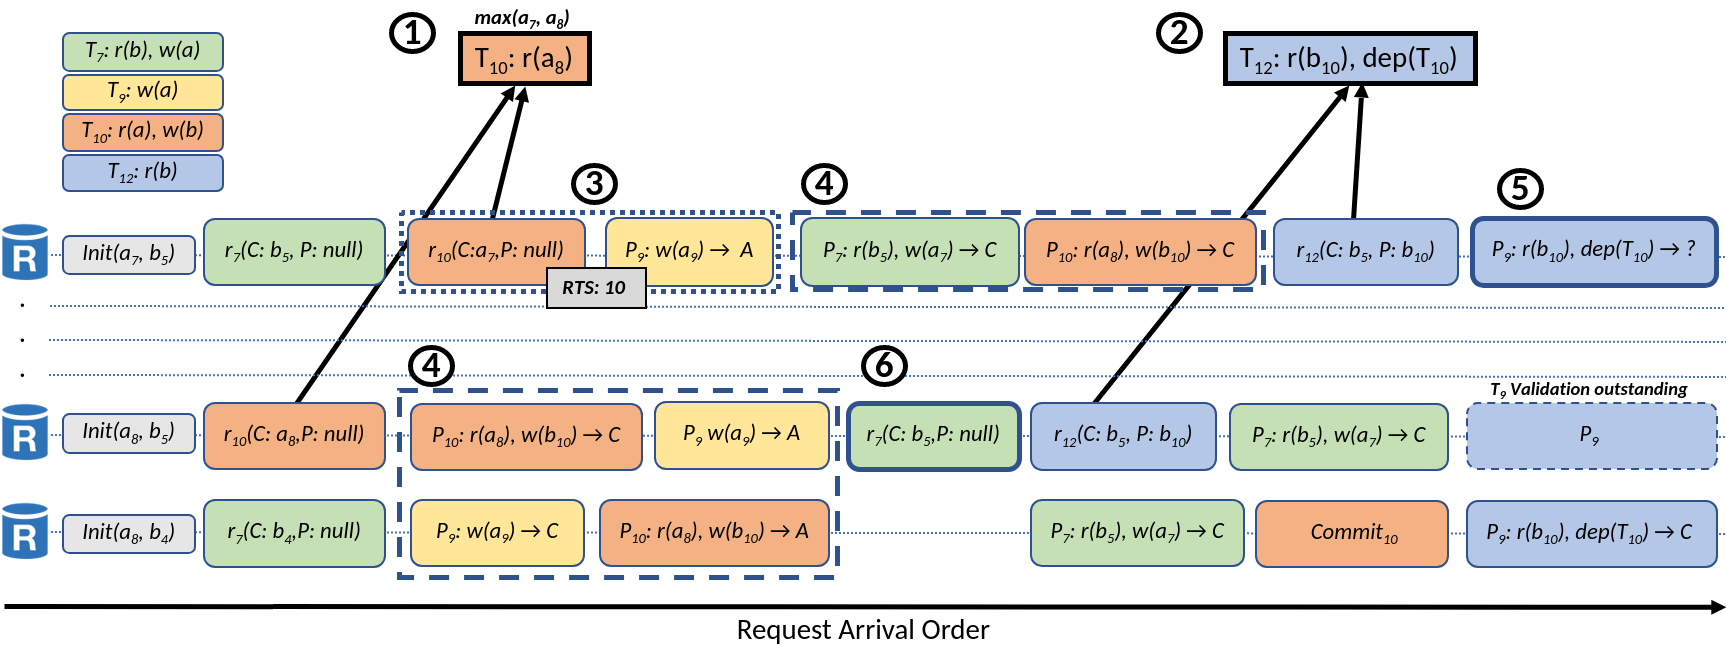
\includegraphics[width= \textwidth]{./figures/MVTSOLargeFont.png}
\end{center}
\caption{\emph{MVTSO behavior for different replica processing orders}. $r_x(C : a_y ,P : a_z)$ denotes that transaction $T_x$ (x being the timestamp of a transaction in this example) reads the version $y$ of object a written by committed transaction $T_y$ and version $z$ from tentative prepared transaction $T_z$. $P_x(RS,WS,DEP)$ denotes a transaction $T_x$'s prepare request (i.e. the validation check) for respective ReadSet (RS), WriteSet (WS) and Dependenc Set (DEP), and $\rightarrow C / A$ denotes the local replica validation outcome (Commit/Abort).} 
\label{fig:MVTSOEX}
\end{figure*}

\par \textbf{MVTSO.} Our starting point is Multiversioned Timestamp Ordering (MVTSO), a concurrency control scheme which prescribes a serialization order by assigning a speculative timestamp \textit{before} execution \cite{bernstein1983multiversion, reed1983implementing, su2017tebaldi}. In MVTSO, read operations return the latest written version smaller than the readers' timestamps. Respectively, writers attempt to create new versions at their timestamp, but must abort if a higher timestamped read would have "missed the write" by reading a prior version. A transaction may commit only, if all read-write dependencies have committed.

\iffalse
\fs{cut the whole following paragraph?} \la{Yes, I would cut it} This allows us to a) only classify concurent read/write operations as conflicting if their execution results violate the timestamp order (Fig. \ref{fig:MVTSOEX}: 4 bottom), and b) avoid write/write conflicts alltogether. 
When speculative execution results match the pre-defined timestamp order, no aborts are necessary (Fig. \ref{fig:MVTSOEX}: 4 top). \sys{}'s challenge is therefore to a) assign appropriate timestamps and b) coordinate execution in a way that maximizes such coherence; the presence of Byzantine participants (clients/replicas) complicates this.

In MVTSO, reads operations return the latest written version smaller than the readers' timestamps, while writers attempt to create new versions at their timestamp, but must abort if a higher timestamped read would have "missed the write" by reading a prior version. A transaction may commit only, if all read-write dependencies have committed.
\fi

When \sys{}'s speculative execution results match the pre-defined timestamp order, no aborts are necessary (Fig. \ref{fig:MVTSOEX}: 4). \sys{}'s challenge is therefore to a) assign appropriate timestamps and b) coordinate execution in a way that maximizes such coherence; the presence of Byzantine participants (clients/replicas) complicates this.

\par \textbf{Byzantine resilience.} Read operations in \sys have the following sub-goals: \one Correct clients should read valid data, i.e. experience read integrity, \two Correct clients should read fresh data, i.e. minimize staleness and hence maximize commit chance, and \three Reads must provide the context necessary to potentially complete observed write state. 
Clients validate the integrity of reads by requiring replicas to provide a proof of validity, which consists of a set of signatures confirming committment, or if not yet existant, a set of  $f+1$ replica's tentative commit endorsements \fs{maybe cut this second part, since it will become redundant}. Moreover, to guarantee that clients do not read maliciously stale data from their local replica, \sys encourages clients to read the latest version across $\geq f+1$ replicas (Fig. \ref{fig:MVTSOEX}: 1,2).
Avoiding Byzantine influence comes at a cost: Read operations require a synchronous, potentially WAN \fs{or just remote - i.e. not local}, rountrip. 

MVTSO intuitively synergizes well with \sys{}'s potenially WAN remote reads as reading from a fixed timestamp helps speculative readers observe consistent snapshots, even when execution is long and consequently interleavings are frequent (Fig. \ref{fig:MVTSOEX}: 6). \fs{at the price of experiencing serializability instead of strict serializability - that is only the case if your timestamps are outdated}.

While we assume that clocks are loosely synchronized across correct participants, Byzantine participants may diverge arbitrarily and propose excessively high timestamps. A simple solution is to bound time-stamps by querying the median time from a Quorum of replicas and including replies as proof \cite{bazzi2004non, bazzi2018clairvoyant}. To side-step the additional overheadd that a dedicated timestamping phase incurs, we compromise by allowing clients to optimistically select their own timestamps, but reject request timestamps above a threshold at all correct replicas, thus incentivising clients to select bounded, close to real-time, timestamps. 

In traditional MVTSO, writes become visible to successive, higher timestamped, reads immediately. However, in the presence of Byzantine clients this is undesirable, as it allows clients to issue write operations without the intention of ever committing a transaction. Thus, any correct clients' read that observes, and consequently depends on a Byzantine clients write may be blocked indefinitely.
%Allowing other clients to preemtively commit outstanding write operations is infeasible, as the remaining transaction procedure is known only to the issuing client, while conceiding pessimistic abort permission empowers Byzantine participants to obstruct any correct clients' writes. 
\sys reconciles this dilemma by deferring all database updates until execution is complete and the client prepares the transaction for commitment. 
% Concretely, \sys clients buffer all write operations, and submit them only when attempting to commit the transaction, thereby enabling other \sys client to orderly complete Validation and Writeback steps.\\
\la{This needs to be better explained} \fs{took a pass:}
Clients in \sys distinguish explicitly between writes \textit{committed} across all involved shards and tentative writes \textit{prepared} at a single shard: While clients accept all verifiable \textit{committed} version from a single replica, they accept \textit{prepared} versions only when endorsed by $f+1$ replicas. This ensures that a) at least one correct replica believes that the write can commit, and hence is worth observing, and b) that Byzantine replicas and clients cannot collude to violate Byzantine independence by reactively inventing versions. \fs{such invented transactions could be designed to be guaranteed to abort: I.e. by claiming to have read an out-dated version. The write versions could be engineered to be perfectly at the bound of the read timestamp, such that it is guaranteed to be chosen}\\
Finally, \sys replicas evaluate writes for conflicts by maintaining a Read Timestamps (RTS) for each locally processed read (Fig. \ref{fig:MVTSOEX}: 3). While this allows un-prepared reads to elicit external effects, these affect only concurrent transactions with smaller timestamps and can be bypassed by re-trying a transaction. To nonetheless limit recurrent abuse, we discuss a personalized lease mechanism to limit Byzantine influence in section Y.z (Optional Modifc). \fs{or just do it here in 1-2 sentences. We do not implement this though.}



\subsection{Execution interface}
Client applications execute transactions via the following interface. A TX object \textit{TXObj $\coloneqq$ (SeqNo, ClientID, InvolvedShards, ReadSet, WriteSet, Dependencies)}, records the state necessary for Validation.

\iffalse
\begin{figure}
\begin{center}
\includegraphics[width= 0.5\textwidth]{./figures/TxState.png}
\end{center}
\caption{Transaction execution state}
\label{fig:Txstate}
\end{figure}
\fi

\textbf{Begin()} A client begins a transaction by optimistically choosing a timestamp \textit{TS $\coloneqq$ (Time, ClientID)} that defines a total serialization order across all clients.  \\
\textbf{Write(key, value)}. A client buffers the write: \textit{WriteSet = WriteSet $\cup$ (key, value)}\\
%%%%%%%%%Read protocol%%%%%%%%%%%
\textbf{Read(key, TS, RQS)} 
If \textit{key $\in$ WriteSet} a client returns the buffered write value. Otherwise, the client conducts a remote read for given hyperparameter Read Quorum Size (RQS):

\fbox{\begin{minipage}{23em}

\textbf{1: C} $\rightarrow$ \textbf{R}: Client sends read request to Replicas
\end{minipage}}\\
%Improve RQS formulation
A client broadcasts a read request  $m = (Read, key, TS)_c$.
\iffalse
 to $RQS$ different replicas. Note, that in order to guarantee $\geq RQS$ replies a client might need to send up to $f$ additional requests to compensate for unresponsive/faulty participants ($max(|Replies|) \leq n-f$). 
\fi
\fs{Optimization: A client sends only to RQS+f to receive RQS many replies}

\fbox{\begin{minipage}{23em}
\textbf{2: R} $\rightarrow$ \textbf{C}: Replica processes client read and replies
\end{minipage}}\\
A replica authenticates the client\footnote{Byzantine replica may ignore read access control. Solving this problem is beyond the scope of this work; we defer to existing solutions \cite{basu2019efficient}.}, and enforces a local timestamp threshold. \fs{this can probably be shortened:} It returns a signed message \text{$\langle \textit{ReadReply, Committed, Prepared} \rangle _R$}, where $Committed \coloneqq (value, version, proof)$ represents the value-version pair with largest committed write version smaller than TS and a proof of commitment,  and $Prepared \coloneqq (value, version, TxID', deps)$ the respective largest uncommitted value-version pair, the associated transaction ID, and the latter transactions potentially uncommitted read-write dependencies. Moreover, a Replica stores a new read timestamp (RTS) for the key: $RTS(key) = RTS(key) \cup TS$ (Fig. \ref{fig:MVTSOEX}: 3). 
\fs{a replica may include a set of prepared values to increase likelihood of client receiving f+1 matching}

\fbox{\begin{minipage}{23em}
\textbf{3: C} ($\rightarrow$ \textbf{R}): Client receives read replies 
\end{minipage}}\\
A client waits for $\geq RQS$ read replies and chooses the biggest valid result \textit{(value, version) $= max_{valid}$(\{Committed\},\{Prepared\}} (Figure \ref{fig:MVTSOEX}: 1,2). A \textit{Committed} tuple is valid, if the proof confirms commitment, wheras a \textit{Prepared} is valid iff there exist $f+1$ matching \textit{Prepared$_r$}. The client adds the version to its read set \textit{ReadSet = ReadSet $\cup$ (key, version)} and additionally claims a dependency if it was a \textit{Prepared} version: \textit{Dep = Dep $\cup$ \{f+1 $\times$ Prepared$_r$ \}} . 

\fs{la: finds the use of commit in both exec and validation confusing. Is it unclear that this refers to application here?}
\textbf{Commit()} A Client terminates its execution, and computes a unique transaction identifier based on final execution object and its timestamp: $TxID \coloneqq (H(TxObj, TS)$, thus preculding Byzantine participants from equivocating transaction contents. It then initiates the Validation Phase by issuing a 2PC-Prepare requests to each involved shard.
%What if a byz doesnt send to all involved shards? It will be visible on some shard and hence an correct client can obtain the full TX. See Hierarchical IDS in Protocol.tex

\textbf{Abort()} A client terminates execution, and broadcasts a request to release all acquired Read Timestamps (RTS). Since writes in \sys are deferred, no other rollback action is necessary.


We briefly discuss some implications of the choice of Read Quorum Size (RQS). Following cases may be distinguished: \one \textbf{$RQS = 1$} A client may read committed data from just \textit{trusted} replica (at the risk of reading stale data) to reduce execution latency and consequently minimize conflicting interleavings. \two \textbf{$RQS \geq f+1$} \sys{}'s recommended minimal mode of operation. While side-stepping maliciously stale reads, it is still possible to read (arbitrarily) stale data due to replica inconsistency, caused by either asynchrony or partial transaction replication by a Byzantine client.
\three \textbf{$RQS \geq \frac{n+f+1}{2}$} When reading from a Quorum of sufficient size to overlap with any Validation Quorum (ref section Validation) in at least one correct replica, a client guarantees, that no more \textbf{additional} (beyond previously observed) conflicting writes can be admitted, since such a Quorum of acquired RTS acts as a read-lock. 

\iffalse
Trusting only $f+1$ matching prepared writes has the beneficiary side effect of allowing us to include only transaction identifiers as dependencies, rather than the full transaction, since it is guaranteed that at least one correct replica has stored the transaction. Thus, in the failure free scenario, where clients need not complete transactions $in Dep$, \sys minimizes the meta-data overhead that the recovery protocol imposes.
\fi

We remark that, consistent with Byz-Isolation, \sys allows Byzantine clients to fabricate and (permissibly) submit arbitrary reads; Byzantine clients may \textit{choose} whether to read legal, or even real data.  \sys does, however, enforce that Byzantine clients cannot (undetectably) fabricate dependencies by requiring a proof of $f+1$ matching prepared writes. This precludes Byzantine clients from indetectibly stalling their own transactions and consequently obstructing liveness for consecutive descendant (second degree...) dependencies.
Furthermore, this allows \sys to include only transaction identifiers as dependencies, rather than the full transaction, thereby minimizing the common path overhead. The full transaction can be acquired from an correct replica when necessary. We discuss how to complete stalled or slow transactions in section Y (Granting Liveness).





%%-------------------------------------------------------------------------------
\subsection{Validation Phase}
%-------------------------------------------------------------------------------

In order to facilitate atomic committment across all shards involved in a transaction \sys clients invoke a Prepare request, inquiring each shard to validate the transaction for conflicts and cast a 2PC vote. Shards in \sys are replicated for fault tolerance.

\fs{idk where to put this and whether to mention at all - but we do want to state that there exists a version with 3f+1 (minimal replication degree) that implements the same ethos }
\sys comes in two different flavors, \sys{}3 and \sys{}5 respectively, that rely on varying replication degrees, but implement the same design. \sys{}3 requires $n=3f+1$ replicas \fs{, the minimum bound necessary for BFT SMR?,} per shard to guarantee consistency in the presence of $\leq f$ byzantine replicas. \sys{}5 reduces both latencies during failure free execution and complexity during recovery. \footnote{We believe that consortiums with high performance requirements or high replication degrees are respectively comfortable with paying for additional replicas or tolerating a lower fraction (1/3 vs 1/5) of failures}
For the simplicity of exposition we discuss \sys{}5 for the remainder of the paper, and defer to section X \fs{and/or TR} to describe differences in \sys{}3. In the following, we outline \sys 's execution (unaffected by replication degree), validation and writeback protocols.

The goals of the Validation phase are threefold: \one It must decide on a single, durable vote per-shard that maintains Byzantine Serializability (henceforth we refer to this as a \textit{shard-decision}), \two It should be leaderless, and not enforce unecessary ordering for commutative, non-conflicting transactions, and \three It must preserve independent operability. \fs{needs to refer to the fallback}

Satisfying these goals requires ovecoming several challenges. In order to maximize parallelism and embrace partial ordering, \sys allows replicas to process requests out of order. Consequently, replicas may temporarily diverge, and hence return different validation results. Such divergence must be reconciled in a way that maintains Isolation, but not overly conservatively in order to bound the impact of byzantine participants and maximize likehlihood to commit. \sys designates clients as validation coordinator for its own transactions, thus omitting a dedicated replica leader. %The respective protocol must tolerate client failures such as crashes, omission/stalling, equivocation, or replays and allow for consistent recovery. 

The Validation protocol can be broken down into two functionalities: Voting and Logging.
Since \sys replicas may process requests in different order, they must reach consensus on a joint  decision. To do so, they cast a vote for their local validation result, which are subsequently democratically aggregated into a decision. In the case of Indicus, the client acts as the transaction coordinator who aggregates and relays results (along with necessary evidence).
In order to maintain consistency in the presence of failures (no two honest replicas finalize different Commit/Abort decisions), this decision must be durable and unique, guaranteeing that a replay of any Writeback is idempotent. However, since a byzantine coordinator cannot be trusted to durably store a decision, nor could we retain liveness during a crash or partition, \sys demands clients to \textit{log} the decision at replicas before returning.
 

The voting step requires a single round-trip to all replicas, whereas the logging phase requires at most one round-trip \fs{in Indicus5 and at most two round-trips in Indicus3.}. When execution is fault- and contention free transactions can be committed on the \textit{Fast-Path} in a single-round trip as an explicit logging round is not necessary.


%%%%%%%%%% protocol
To describe how the protocol operates in detail we follow a single-shard transaction through the system:

\fbox{\begin{minipage}{23em}
\textbf{(1: C $\rightarrow$ R)}: Client sends Prepare request to all Replicas within the Shard.
\end{minipage}}\\
Upon deciding to Commit in the Execution phase, a Client initiates Validation by sending a message $Phase1 \coloneqq \langle Prepare, TxID, TX \rangle_{\sigma_c}$ to all Replicas.

\fbox{\begin{minipage}{23em}
\textbf{(2: R $\rightarrow$ C)}: Replica receives validation request, processes it and returns vote to Client.
\end{minipage}}\\
A replica validates Timestamp and Dependency integrity of the request. It then evaluates Read and Write Sets for Isolation conflicts against its local state using the MVTSO Concurrency Control Check (CCC), as shown in algorithm 1. It returns a message $Phase1R \coloneqq \langle TxID, vote \rangle_r$, and optionally evidence in case it voted to Abort.

\underline{Additional subtlelties}: 
A replica never changes its Voting decision, because re-execution could leave to different results. Once the MVTSO-Ceck completes (i.e. there are no blocking dependencies), a replica starts a timer to monitor the clients progress.

\fbox{\begin{minipage}{23em}
\textbf{(3: C)}: Client waits for vote replies.
\end{minipage}}\\
A client waits for at least $n-f$ ($4f+1$ in Indicus5) distinct replica votes, or more, up to a system specified timeout. 

\fbox{\begin{minipage}{23em}
\textbf{(3a: C)}: Client receives Threshold of matching votes and returns to application. Proceeds to Writeback
\end{minipage}}\\
In any of the following 3 cases, a client may short-circuit waiting for additional votes and omit a dedicated Logging round:
\begin{enumerate}
\item \textbf{$1$ Abort vote w/ Conflicting TX \& CommitCertificate}: A conflict with a commited transaction. The client validates the integrity of the CommitCertificate and returns the shard decision $(TxID, Abort, \langle ConflTX \rangle_{CC})$. 
\item \textbf{$3f+1$ Abort votes w/ Conflicting TX}: A conflict with a prepared, but not yet committed transaction. The client returns the shard decision $(TxID, Abort, \{\langle AbstainVote\rangle_r\})$. 
\item \textbf{$5f+1$ Commit votes}: No conflicts. The client returns the shard decision $(TxID, Commit, \{\langle CommitVote \rangle_r\}$
\end{enumerate}
Any of such Quorums forms a \textit{Shard-Certificate} and proves the decision. A client uses this Certificate to return to its application and issue the Writeback.

\fbox{\begin{minipage}{23em}
\textbf{(3b: C $\rightarrow$ R)}: Client receives divergent results and suggests a consistent decision to Replicas for Logging
\end{minipage}}\\
If a client does not receive the necessary thresholds of votes to return, it must continue on the \textit{Slow-Path}. To do so, it aggregates the votes according to following decison rule:
If there exists a $CommitQuorum \coloneqq \frac{n+f+1}{2}$ of Commit Votes, the Slow-Path decision is Commit, otherwise it is Abort.
A client broadcasts a message $Phase2 \coloneqq (TxID, decision)_c, \{\langle votes \rangle_r\}$.

\underline{Additional subtlelties}: A client forwards a Quorum of $\geq n-f$ votes to the replicas in order to prove the Slow-Path decision is consistent with Isolation guarantees. Note, that a byzantine client may equivocate the decision by relaying different Quorums.

\fbox{\begin{minipage}{23em}
\textbf{(4: R $\rightarrow$ C)}: Replicas receive, validate and echo decision
\end{minipage}}\\
A replica confirms that the Decision matches the Quorum by evaluating the decision rule itself and adopting the decision. It then returns the decision to the client by sending $Phase2R \coloneqq \langle TxID, decision \rangle_r$. Importantly, a replica never changes its decision.

\fbox{\begin{minipage}{23em}
\textbf{(5: C)}: Client returns shard-decision to application and proceeds to Writeback
\end{minipage}}\\
A client waits for a Quorum of $n-f$ matching $Phase2R$ messages. Such a Quorum forms a \textit{Shard-Certificate} and proves the decision. A client uses this Certificate to return to its application and issue the Writeback.

\underline{Additional subtlelties}: If a client equivocated, it will never receive a Shard-Certificate. An honest client however, is guaranteed to receive matching Phase2 replies. 

We consider a decision (Commit, Abort) to be \textit{logged} when it is possible for some Shard-Certificate to exist, i.e. as soon as the necessary certificate Quorums exists at some Replicas.
Figure \ref{fig:FigureSP} summarizes the relevant nomenclature.

\begin{figure}
\begin{center}
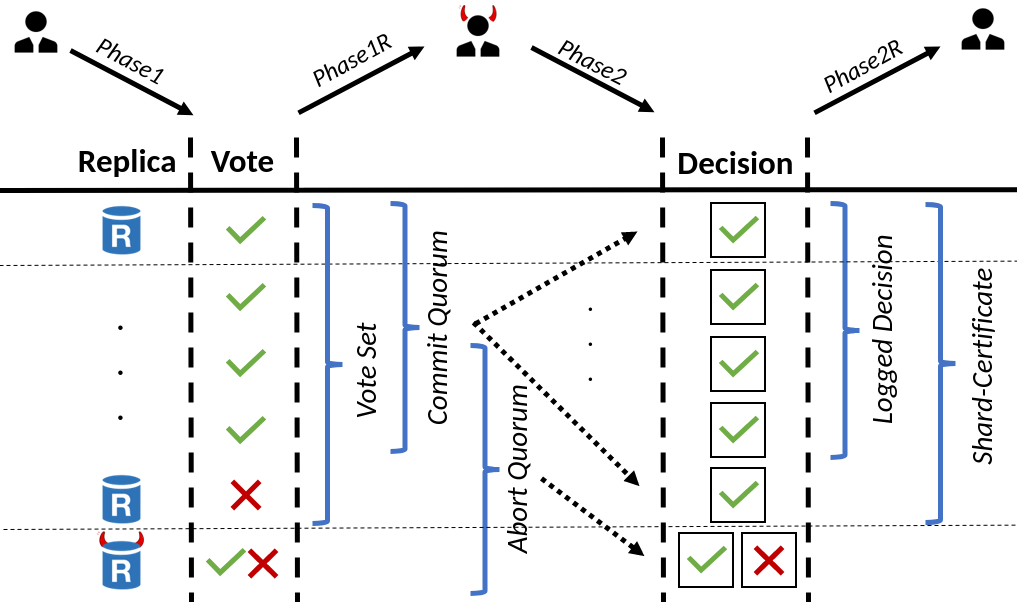
\includegraphics[width= 0.5\textwidth]{./figures/Nom2.png}
\end{center}
\caption{Validation Nomenclature, Slow-Path. Note, that a byzantine client may equivocate Phase2 decisions by including Commit and Abort Quorums respectively. Byantine replicas may store multiple votes and decisions.}
\label{fig:FigureSP}
\end{figure}

\subsubsection{Correctness}
We show, that a \textit{logged} decision is final:
\begin{theorem}[Saf]
A logged decision is durable, and there can ever exist \textbf{at most one} logged decision.
\end{theorem}
\begin{proof}
See TR.
\end{proof} 

Note, that since replicas never change their decision, it is possible for there to never be any logged decision if a byzantine client equivocated its Slow-Path Quorums. In order to reconcile this, we design and discuss a recovery mechanism in section X which relaxes the requirement on persisting a decision.  


\begin{theorem} 
Indicus maintains \textit{Byzantine-Serializability}.
\end{theorem}
To prove that this is the case, we show that for any two conflicting transactions, at most one can be committed.
\begin{proof}
See TR.
\end{proof}

\begin{theorem} 
Indicus maintains Byzantine Independence in the absence of network adversary.
\end{theorem}

We show, that once a Client submits a transaction for validation, the result cannot be unilaterally decided by any byzantine participant, be it client or replica.
\begin{proof}
See TR.
\end{proof}
%
\subsection{Validation Check}

Algorithm \ref{mvtso} shows the necessary validation check to preserve Byzantine-Serializability. 
Given a transactions prepare request the validation check returns an Abort vote if a conflict has been detected, and Commit otherwise. 
When execution results match the timestamp order, there are no conflicts (Fig. \ref{fig:MVTSOEX}: 4 top). For each read, a replica verifies that it has not voted to commit a conflicting write (Algorithm \ref{mvtso}, line 3-7). Conversely, for each write, a replica confirms that there exist no previously accepted reads (line 8-10), and no ongoing read transactions (line 11-12) that conflict. Fig. \ref{fig:MVTSOEX}: 4 shows both non-conflicting and conflicting interleavings.
If there are no conflicts, a replica tentatively \textit{prepares} a transaction, making its writes visible and evaluating future transactions against it for conflicts. Regardless of the outcome, a replica garbage collects all Read Timestmaps (RTS) associated with the transactions reads.
It then waits for necessary dependencies (uncommited writes that were read) to be resolved (Figure \ref{fig:MVTSOEX}: 5). We remark, that the concurrency control check is serialized and executed atomically for each transaction.

\begin{theorem}
The set of transactions for which the MVTSO-Check returns Commit is Byzantine-Serializable. 
\end{theorem}
\begin{proof}
See TR.
\end{proof}

\begin{algorithm}
\caption{MVTSO-Check(TX, TS)}\label{mvtso}
\begin{algorithmic}[1]
\If{\textit{$TS > localClock + \delta$}} %  || $TS < lowWM$ || $\exists d \in dep: d.TS < lowWM$} } dont mention garbage collection part here, it only confuses
\State \Return Abort
\EndIf

\For{\textit{$\forall key,version \in \textit{TX.RS}$}}
        \If{$ \exists TX2 \in Committed \cup Prepared: key \in \textit{TX2.WS} $ \newline
        \hspace*{2em} $\land \, version < \textit{TX2.TS} < TS$}  
          \State  \Return Abort, \textit{TX2, (TX2.CommitProof)}  
         \EndIf  
\EndFor

\For{\textit{$\forall key \in \textit{TX.WS}$}}
        \If{$\exists TX2 \in Committed \cup Prepared:$ \newline 
        \hspace*{2em} $\textit{TX2.RS[key].version} < TS < TX2.TS$} 
          \State  \Return Abort, \textit{TX2, (TX2.CommitProof)}
         
        \EndIf
        \If{$\exists RTS \in key.RTS: RTS > TS$} 
          \State  \Return Abort
       \EndIf
\EndFor
\State Prepared.add(TX) 

\While{$\exists d \in dep: d \notin CommitLog \cup AbortLog $)}
\State Suspend
\EndWhile

%structure it in a way that is better
\For{\textit{$\forall d \in dep$}}
		\If{$ d \in AbortLog $}
		\State	Prepare.remove(TX)
		\State \Return Abort, \textit{(TX2.AbortProof)}
		\EndIf
\EndFor
\State \Return Commit
\end{algorithmic}

\end{algorithm}

In order to perform the MVTSO-check, a replica maintains several data strucutres: \one It stores read timestamps, read versions alongside the multiversioned write stores for committed and tenative transactions respectively, to provide efficient evaluation of conflicts.
\two In order to confirm dependency outcomes, replicas log proofs for completed transactions in respective Commit and Abort Log sets, that together induce the ledger of all processed transactions. 
\three To avoid busy waiting when dependencies are not yet resolved, a replica temporarily suspends the MVTSO-check for the current transaction, allowing it to process other transactions pending validation. To facilitate this, it keeps track of an additonal transaction to dependents mapping that allows to identify and resume all suspended MVTSO-checks associated with dependents of a completing transaction.

\iffalse

\textit{Aside:} Consistent with our definition of Byzantine-Isolation, byzantine clients may issue ficticious Read-Sets comprised of arbitrary read versions and values. However, these have only limited external effect on concurrent writes. We distinguish two extreme cases: 1) $read.version \rightarrow 0$: This case is equivalent to simply reading stale data, and effectively reduces MVTSO to TSO as conlflicts are evaluated only on basis of the transaction timestamps (i.e. Abort write if: write.TS < read.TS). 2) $read.version \rightarrow read.TS$: In this case there are no conflicts as a write is never "missed" by a previous read.
\fi

In the following section we will show how to design a replicated validation scheme that upholds Isolation guarantees and reaches a single shard decision, even when replicas within a shard validate in different orders.

%%-------------------------------------------------------------------------------
\subsection{Consistent logging.}
%-------------------------------------------------------------------------------
Principles and challenges

protocol overview: pic

%%-------------------------------------------------------------------------------
\subsection{Writeback}
%-------------------------------------------------------------------------------



%\subsection{Multi-sharding}

and Multi-shard 2pc

- Optimization: Single shard logging

%%-------------------------------------------------------------------------------
\subsection{Failures}
%-------------------------------------------------------------------------------
- Fallback: election (only starts if not waiting on another dep to avoid early eviction), views, resolution, subtelties with mvtso (block because of dep), necessity even without dependencies. Interested clients, write-back multishard. garbage collection
- Fallback requires an extra round in order to learn about current views to start viewchange, but thats ok: Its co-function with learning about full TX, and checking for existing certificates. Timeout invocation is concurrent with p1 message.

%%-------------------------------------------------------------------------------
\subsection{Low Cost mode}
%-------------------------------------------------------------------------------
3f+1 if not defending against byz colluders
OCC if not worried about reads aborting


%-------------------------------------------------------------------------------
\section{Protocol}
%-------------------------------------------------------------------------------
Indicus comes in two different flavors, Indicus3 and Indicus5 respectively, relying on varying replication degrees. Indicus3 requires 3f+1 replicas per shard to guarantee consistency, the minimum bound necessary for BFT SMR. Indicus5 uses a higher replication degree of 5f+1 replicas, but in return brings down both gracious execution latency and complexity during uncivil executions. We argue, that unlike past system settings where a single authority strives to maintain the fewest amount of replicas necessary for cost considerations, consortium systems with naturally higher replication degree are willing to pay the additional price for performance. Moreover, rather than trying to reach the threshold of replicas to tolerate some number of faults, these settings may start with a fixed number of replicas and consider the ratio of faults to be tolerable. When argueing from this perspective, the perceived difference between tolerating 1/3 and 1/5 of replica failures may be negligible.
For the simplicity of exposition we outline Indicus5 in detail below. In section X we describe the differences in Indicus3.


%%%%%%%%%%%%%%%%%%%%%%%%%%%%%Figs
\begin{figure}[t]
  \begin{mdframed}[roundcorner=10pt]
 	\textbf{TX Exec State}
 	\begin{itemize}
 	\item ClientID
 	\item ClientSeqNo
 	\item InvolvedShards = \{S\}
 	\item ReadSet = \{(key, version)\}
 	\item WriteSet = \{(key, value)\}
 	\item dependencies = \{$\langle (key, version, \{TxID'\})_{f+1 \sigma} \rangle$\}
 	\item TxID = H(TX)
 	\item Timestamp = (Time, ClientID)  optional:, TxID) this is just deterministic tie breaker when a client misbehaves.
 	\end{itemize}
  \end{mdframed}
  \caption{Transaction Execution state}
  \label{fig:TX}
\end{figure}

\newcommand{\SubItem}[1]{
    {\setlength\itemindent{15pt} \item[-] #1}
}

\begin{figure}[t]
  \begin{mdframed}[roundcorner=10pt]
 	\textbf{Replica }
 	\begin{itemize}
 	\item ReplicaID
 	\item ShardNo
 	\item LocalClock
 	\item RTS = \{(key, \{(TS, \{dep\})\})\}
 	\item Ongoing:
 	\subitem OngoingTX = \{(TxID, [TX, val state])\}
 	\subitem PreparedDB = \{(key, [writes:\{(val, version, TxID)\},  reads: \{TS, rversion, dep, TxID\}])\}
 	\subitem WaitingDeps = \{(TxID, dependents\}
 	\subitem Deps = \{(TxID, dependencies\}
 	\item DB = \{(key, [w: \{(val, ver, TxID)\}, r: \{(TS, rv, TxID)\}])\}
 	\subitem CommitLog = \{(TxID, CommitCert)\}
 	\subitem AbortLog = \{(TxID, AbortCert)\}
	 	
 	
 	\end{itemize}
  \end{mdframed}
  \caption{Replica State and Datastructures}
  \label{fig:RS}
\end{figure}


\begin{figure}[t]
  \begin{mdframed}[roundcorner=10pt]
 	\textbf{TX Val State}
 	\begin{itemize}
 	\item TxID
 	\item originalClientID
 	\item interestedClients = \{CID\}
 	\item ClientSeqNo
 	\item Transaction = TXExecState
 	\item vote   ~~~~~~~~~~//Prepare1R
 	\item decision = (dec, view.no) ~~~~~~~//Prepare2R
 	\item optional: dec proof = \{$votes_r$ \} ~~~ //Only for Retries and Indicus3
 	\item current.view
 	\end{itemize}
  \end{mdframed}
  \caption{Transaction Validation State at Replicas}
  \label{fig:TX}
\end{figure}

%-------------------------------------------------------------------------------
\subsection{Execution}
%-------------------------------------------------------------------------------
Clients in Indicus both execute and submit their own Transactions. As previously defined a Transaction TX is a sequence of read and write requests that is ultimately terminated by a Commit or Abort decision. A TX object, as shown in Figure \ref{fig:TX} records the execution state necessary for Validation. The execution protocol has three goals: 1) Honest Clients should read valid data, i.e. experience read integrity, 2) Honest Clients should read fresh data, i.e. minimize staleness and hence maximize commit chance, and 3) avoid expensive coordination as much as possible. This is complicated by the presence of byzantine replicas as well as concurrent transactions. Byzantine replicas may provide invalid or arbitrarily stale data and honest replicas may be temporarily out of sync.

We avoid invalid reads by requiring replicas to provide a proof of validity, i.e. a Quorum of Writeback signatures confirming the committment, or alternatively, trusting only $f+1$ matching replies from discrete replicas. In order to minimize coordination only read requests incur a network rountrip, while writes are buffered locally until Validation. 
Since together Validation and Writeback together incur several Wide Area Network (WAN) message delays, a committing transaction is invisible to concurrent transactions for the time-being, yet results in isolation conflicts that need be resolved. In order to minimize this window, we allow transactions to speculatively read proposed, yet uncommitted values. Similarly, since Execution can span multiple read requests that require WAN message delays, there remains a potentially large period in which reads are vulnerable to conflict. To mitigate aborts due to write conflicts, we a) let reads be sequenced at a pre-defined timestamp (rather than always reading the most recent) and b) let reads acquire implicit read-locks that disallow conflicting writes. 

\fs{lead over to MVTSO - what I just described are the three base techniques}



Client execution conducts as follows:

\begin{enumerate}
\item \textbf{Begin} A client begins a Transaction by optimistically choosing a timestamp $TS \coloneqq (Time, Client ID)$. 
\item \textbf{Write(key, value)}. A Client executes a request Write(key, value) by locally buffering (key, value) and returning. Concretely: $WriteSet = WriteSet \cup (key, value)$

%%%%%%%%%Read protocol%%%%%%%%%%%

\item \textbf{Read(key, TS, RQS)} 
\fbox{Client does blabla}
\fbox{\begin{minipage}{21em}
\textbf{1: C} $\rightarrow$ \textbf{R}: Client sends read request to Replicas
\end{minipage}}

Given hyperparameter Read Quorum Size (RQS), a Client performs a read on given key at timestamp TS by reading from RQS different replicas. To do so, a Client sends $\langle(CID, key, TS)\rangle_{\sigma_c}$ \fs{technically CID is part of TS} to the respective replicas.\\

\fbox{\begin{minipage}{21em}
\textbf{2: R} $\rightarrow$ \textbf{C}: Replica processes Client read and returns reply
\end{minipage}}

A replica returns a signed pair \text{$\langle \textit{(Committed, Prepared)} \rangle _{\sigma_r}$}, where Committed is the write with largest committed write version prior to the specified Timestamp and Prepared is the respective largest uncommitted write that might be committed and would make Committed outdated. 

\underline{Additional subtlelties}: If the timestamp is beyond a Highwater mark ($HW = localClock + \delta$) replicas ignore the requests. If the request is serviced, a Replica adds the timestamp to its Read Timestamp Set (RTSS): $RTSS(key) += (TS)$. \text{$Committed \coloneqq (value, version)_{cert}$} such that $ (value, version) \in R.CommitLog$, $version = max(q) : (key, val, q) \in R.CommitLog \land v < TS \}$ and $cert$ is a certificate proving (value, version) was legally committed (see Section Writeback). $cert$ does not need to be signed by the replica, as it aleady consists of replica signatures.
 $Prepared \coloneqq (value, version, dep)$ such that $(value, version) \in R.PreparedSet$, $version = max(q) : (key, val, q) \in R.PreparedSet \land Committed < v < TS \}$ and $dep$ is a DAG of Transaction IDs, starting from the TX that wrote $(value, version)$ and extending to its own dependencies.
\fs{A replica does not return Prepared, if the uncommited transaction producing the write is still waiting on its own respective dependencies. This avoids the potenial for chain existance with multiple byzantine clients which could violate Byzantine Independence and increases the risk of cascading aborts. In this case one does not need a DAG, because there exist only direct deps}

\fs{A replica only does this, if the client has access control for the value. (limits ability of byz clients to claim dependencies - they can always read from byz replicas if we dont require multi party ocmputation/secret sharing, which is beyond the scope)}


\fbox{\begin{minipage}{21em}
\textbf{3: C} ($\rightarrow$ \textbf{R}): Client receives read replies and asynchronously dissipates dependencies
\end{minipage}}

A client waits for RQS read replies and validates the integrity of any $Committed$ it receives.  It adds the biggest $Committed$ or $Prepared$ (iff enough matching) version seen to its Read Set, and claims a dependency if it was a $Prepared$ version. If it claims a dependency, it asynchronously forwards this dependency to all replicas. 
\{send dependency set, does not need to be proven.\}


\underline{Additional subtlelties}: If $RQS > n-f$ a Client waits only up to a application set timeout beyond the first $n-f$ received replies. If $f+1$ matching $Committed$ are received they need to be validated. If $f+1$ matching $Pepared$ are received from disjoint replicas, and
 $Prepared.version > max(\{Committed.version\}, \{\langle Prepared.versions \rangle_{f+1 \sigma_r}\})$ the client adds Prepared to its Read Set and claims a dependency by including the $f+1$ signatures: $ReadSet += (key, Prepared.version)$ and $dependencies += \langle Prepared.dep \rangle_{f+1 \sigma_r}$. A client then broadcasts a message $Except \coloneqq \langle (key, TS, dep)\rangle_{\sigma_c}$ to all replicas. 
\fs{Receiving f+1 matching might not be possible if there are a lot of concurrent writes that have prepared - out of order for example - to reconcile this, replicas could send a set of s latest writes. Then a client needs to match the largest for which it can find f+1 matching in the sets. This increases overhead (this message must also be forwarded in the deps)}
\fs{does the value need to be included?} 
If there exists no such Prepared, it adds the largest valid Committed, i.e. $ReadSet += (key, max(Committed.version)$. 
\fs{waiting for f+1 allows us to Not include the whole TX, as we are guaranteed to "find" it based on the Txid if we need it later, this is a lot more efficient. (especially if dep trees can grow exponentially). Furthermore, it guarantees us that the TX was not reactively forged in a manner that is guaranteed to abort. The TX must have been there "first". Lastly, we dont want byz clients to claim on less than f+1, because then we could not verify in hindsight that the above 2 properties were upheld inductively. Lastly, f+1 gives you some amount of confidence that this is a transaction that "could" commit (no guarantee), at least one  honest replica believes so. Aborts are then due to normal contention, and not due to byzantine misbehavior}


\fbox{\begin{minipage}{21em}
\textbf{(4: R)} : Replica receives dependencies and adds exceptions
\end{minipage}}
Upon reception of $\langle (key, TS, dep)\rangle_{\sigma_c}$ a replica adds an exception to its Read Timestamp Set. Concretely, $RTSS(key)(TS) += dep$.

\underline{Additional subtlelties}: the dep set received does not need to have proofs, since a client is only trying to gain additional protection by allowing dependencies to be committed. If this set is "fake", it will only cause the own read to abort later, because more writes than desired were allowed to pass. "It just weakens the power of the read lock", which is not relevant for safety, but only for commit rate.
(does one need a check in MVTSO that deps are correct? If max depth =1, then one does not need to send deps anyways, because byz can always lie; or is it still necessary to finish with fallback)
A: byz client only includes dependencies to avoid direct fallback eviction. Only by including proof for deps can it be validated, that these deps are real and can be traced in order to induce a fallback on them)



\item \textbf{Commit} A Client finalizes its execution, computes the final $TxID \coloneqq H(TX)$  and submits the Transaction for validation.

\underline{Additonal subtlelties}: Computing the transaction identifier based on a hash of the execution object guarantees that a byzantine client may not equivocate transaction contents. The ID serves both as common identifier for remaining protocol components, and as validation tool for the integrity of a transaction object.

\item \textbf{Abort} A client terminates execution, broadcasts a read-release for all potentially acquired Read Timestamps (RTS) and returns.

\underline{Additonal subtlelties}: A byzantine client may never release its RTS. For instance, it may perform reads just for the sake of acquiring RTS without any intention of committing. We discuss mechanisms to sidestep this in section X (Optional Modifications).

\end{enumerate}

\fs{Need to talk about MVTSO here first}
 
We briefly discuss some implications of the choice of Read Quorum Size (RQS) as well as the general MVTSO design.
 
A client may choose to read from any number of replicas. Following cases may be distinguished:
\begin{itemize}
\item \textbf{$RQS = 1$} A replica may read from just 1 replica at the risk of later aborting due to reading maliciously stale data (i.e. replica claiming no write ever existed). Note, that an honest client is still guaranteed to read valid data, as only Committed reads are processed. If a Client trusts a local replica \textbf{and} the replica is not lagging behind, this is a viable option to reduce execution time and hence improve both latency and conflict likelihood.
\fs{Alternatively: Read from f+1 matching always without certificate to reduce proof/memory costs: Could not get matching and hence fail read. Still possible to abort by reading stale data}
\item \textbf{$RQS \geq f+1$} When reading from $f+1$ or more replicas a client is not susceptible to maliciously stale reads, yet it is still possible to read (arbitrarily) stale data, either due to inconsistency caused by asynchrony or a byzantine client not fully replicating its transaction. Furthermore, it is always possible to miss a concurrent TX in the pipeline.
\item \textbf{$RQS \geq \frac{n+f+1}{2}$} When reading from $3f+1$ (in Indicus5, or $2f+1$ respectively in Indicus3), a client guarantees, that no more \textbf{additional} conflicting writes can be admitted, since such a Quorum acts as a read-lock. If a single Prepared write would suffice to form a dependency \fs{this would also require sending the whole TX and not just TXid in order for an honest client to be able to start the fallback if necessary}, then it would be guaranteed, that a read cannot abort, since the freshest possible value would have been read \fs{all smaller reads would have either been seen or will abort}. This however, overly empowers byzantine replicas:  Depending on such transactions is undesirable, as there exists neither confidence that this transaction does not violate Isolation, nor would \textit{Byzantine Independence} be upheld as byzantine replicas could reactively fabricate transactions that are guaranteed to abort. Thus, we require a read dependency to only be formed on $f+1$ or more matching replies. Note, that this does \textbf{not} guarantee that a read did not miss concurrent writes, but provides a reasonable trade-off.
\fs{A client could decide to wait for even more matching replies in order to increase confidence that the TX will commit. However, only if he receives $5f+1$ this would be guaranteed.}

\fs{- also has the effect of not needing to store the full TX always, because one honest is guaranteed to have it and we can get it later.
- Byz clients could fabricate their own dependencies }
\end{itemize}





Exceptions: granting exceptions is protection for oneself: minimize the window of dependent writes aborting against oneself. \fs{Should not rely on deps beyond depth 1, because those could be both byz and not claim exceptions and abort themselves always}

(Note : the TS used here is not the final one, its just the tuple of time and clientId. (The triple later is just necessary to differentiate two TX by a client that were assigned the same Time
)



- Read proofs required for honest client correctness. Alternatively one can read from f+1 only, but that can result in failed/older reads

- Notice, that a byz client does not follow this protocol. It can do whatever reads it wants, but it cannot claim non-existant dependencies. Do not need to include read proofs in the prepare. According to Isolation definition byzantine Clients can read whatever they want. Moreover, Reads only have very limited external effect. The value does not matter for the CC check. The version has bounded effect: If it goes towards 0, then it is just a check between timestamps as normally. If it goes towards the TS, then it will never abort.

- Fallback not just useful for dependency cleanup, but also "unclaimable" concurrent TX that need to finish.

\fs{
1. read access control not possible since 1 byz can return write. This requires Multi party computation, shared secrets (verifiable secret sharing), beyond the scope of our work (reference soumyas paper)
2. need to be clearer on the byz independence violation when single read deps are allowed. Byz clients could fabricate their own dependencies 
}



%-------------------------------------------------------------------------------
\subsection{Concurrency Control}
%-------------------------------------------------------------------------------
Next, we discuss the concurrency control necessary to maintain Byzantine-Serializability. Since Indicus clients execute optimistically concurrently Isolation conflicts might arise. In order to reconcile conflicts we need to design an appropriate Validation check that assures that no two conflicting transactions may commit. In this section we discuss the design of our concurrency control check (CCC). In section X (Validation) we then we discuss how to coordinate this check in a replicated but on-ordered setting.

\fs{this text is a hot mess and needs to be reworked. How to express concisely why we want our MVTSO design. Avoid redundancy with previous section. Does this need to come inbetween?}
The goal of the concurrency control mechanism is to maximize the legal commutativity between transactions (i.e. maximize commit rate for concurrent transactions) while maintaining the desired Isolation level, Byzantine-Serializability. A naive Optimistic Concurrency Control (OCC) mechanism pairwise evaluates any two concurrent transactions and classifies any concurrent read/write, write/read, write/write as a conflict. Aborting every conflict preserves safety, yet is often overly pessimistic and could be avoided by a simple re-ordering of transactions. Such could either be achieved in hindsight, i.e. by forming and evaluating a DAG of transactions, or by optimistically pre-defining an order.
Our starting point is a traditional Timestamp Ordering approach (TSO) in which each transaction is assigned a speculative timestamp \textit{before} Validation. This allows us to a) evaluate read/write conflicts on the basis of their pre-defined order, i.e. only classify them as conflict if their arrival order violates the timestamp order, and b) avoid write/write conflicts alltogether by simply ignoring obsolete writes (Thomas Write Rule). 
When execution results match the pre-defined timestamp order, no aborts are necessary. Our challenge then becomes to 1) assign appropriate timestamps and 2) coordinate execution in a way that maximizes such coherence; the presence of byzantine participants (clients/replicas) complicates this.

1) First, we require a timestamping service that (accurately) reflects the real-time execution start. While we assume that clocks are loosely synchronized across honest participants, byzantine participants may diverge arbitrarily in undesirable fashion. Read transactions with timestamps that are too far in the future can cause all successive "younger" transactions to abort. 
A straightforward way to bound legal timestamps is to rely on a verifiable timestamping phase: A client may query a Quorum of $\geq 2f+1$ replicas for their local time and choose the median which provably bounds byzantine timestamp divergence. This however, entails an extra WAN Roundtrip, increases observed clock divergence due to different replica latencies and requires attaching a Quorum of signatures. To side-step this additional overhead we compromise by allowing clients to optimistically select their own timestamp, but rejecting timestamps above some Threshold. We point out, that both choosing a timestamp that is too small or too large increases the risk of ones own transaction being ignored, thus incentivising clients to select real-time timestamps. In order to facilitate a total serialization order across all clients, we define Timestamps to be tuples of the form $(Time, CID)$. A byzantine client however, may choose identical timestamps for two different transactions. Such ties can be broken by TxID order. Furthermore, this is an observable misbehavior: A replica can safely dency processing from the second transaction received and report the issuing client.

2) Second, in order to maximize coherence between execution and timestamp we desire to minimize both execution and commit (validation \& writeback) time. The smaller the window for out-of-order interleavings, the higher the rate to commit. As previously alluded to, writes are buffered locally, while reads may require WAN roundtrips to provide integrity. This increases the window for conflicting writes to arrive, thus causing read transactions to abort.
Moreover, achieving replication (Validation/Writeback phase) requires additional roundtrips in order to maintain consistency. Consequently, write transactions become committed only after a long time, resulting in successive concurrent reads arriving out-of-order.
To mititage the frequency of read aborts we add three mechanisms on top of TSO:
\begin{itemize}
\item Multiversioning: We store multiple past write versions and allow read transactions to "read in the past". This avoids unecessary aborts when read transactions execute only \textit{after} a write with higher timestamp. Previously, long executing read transactions (i.e. multiple sequential reads) could have suffered from their timestamp growing smaller and smaller relative to concurrent write transactions validating at the same times.
\item Read Uncommitted: We allow read transactions to optimistically read partially validated, but not fully committed transactions. By making writes \textit{visible earlier}, unecessary aborts for reads that would have previously missed the newer write are avoided.
\item Read Timestamps: We allow read ransactions to claim \textit{Read Timestamps} by signaling replicas to abort out-of-order writes (writes with smaller timestamps). This fairness policy implements a bias towards read transactions, by aborting writes instead of reads. Since most workloads are read dominated and write-only transactions can re-execute more swiftly, this is an intuitively sensible trade-off. In section Y we discuss an optional modification to support read-modify-write transactions. \fs{retries}
\end{itemize}

\fs{Note, that if there is no concurrency, then MVTSO degenerates to TSO.}

Algorithm \ref{mvtso} shows the necessary validation check to preserve Byzantine-Serializability. 
Given a transaction TX finalized execution state, i.e. its read-set, write-set and dependencies, and a proposed timestamp, the validation check returns \textit{Abstain/Abort} (we discuss the distinction further in section X (validation)) if a conflict has been detected. Otherwise, a replica tentatively \textit{Prepares} a transaction by adding its reads and writes to the $PreparedDB$, making its writes visible and evaluating future transactions against it for conflicts. It then waits for necessary dependencies (uncommited writes that were read) to be resolved. \fs{should unprepare if dep aborts; this avoids more dependencies to be formed unecessarily}
If all dependencies resolve do so successfully the check returns Commit, and otherwise un-prepares the transaction and returns Abstain/Abort. We remark, that the concurrency control check is serialized and executed atomically for each transaction.

\paragraph{Replica State}
\fs{Need to modify MVTSO pseudocode to match the replica strucutres? or is the way it is expressed rn better.}
In order to perform the MVTSO-check (efficiently), a replica maintains several data strucutres as seen in Figure \ref{fig:RS}): It keeps track of its \textit{Database}, of \textit{Ongoing} transactions, and \textit{Completed} transactions. The Database is manifested as multi-versioned key value store. It contains both the writes and reads of all committed transactions.
Further, completed transactions are logged in respective Commit and Abort Logs, that effectively represent the ledger of all processed transactions. Since replicas process transactions out of order, we store this log as a set. This allows us to perform swift lookups for dependencies as transactions can be identified by their TxID. 
Replicas keep track of ongoing transactions and their respective validation protocol state (see section Y). Additionally, it maintains a temporary key-value store $PreparedDB$ of tentatively committing (prepared) transactions to service both optimistic reads and check for conflicts. 
When a transaction performs the MVTSO-check, its dependencies may not yet be present in either Commit or Abort logs. To avoid busy waiting, a replica temporarily suspends the MVTSO-check for the current transaction until all dependencies are resolved, allowing it to process other transactions pending validation. To facilitate this, a replica keeps track of two additional datastrucutres, \textit{WaitingDeps} and \textit{Deps}. WaitingDeps maps a transaction to all its known dependents, i.e. for a transaction TX1 with dependencies \{TX2, TX3\} WaitingDeps contains two entries (TX2: \{TX1\}) and (TX3: \{TX1\}). Vice versa, Deps, contains all unresolved dependencies for a given transaction, i.e. (TX1: \{TX2, TX3\} in the given example. When a transaction (e.g. TX2 completes) a replica can search Waiting Deps to find all of its dependents, and update the dependents Deps set accordingly. A replica may then resume a suspended MVTSO-check for transaction TX by either Abstaining/Aborting if a dependency was added to the AbortLog, or returning Commit if $Deps[TX]$ is empty.
In section X (Writeback) and Y (Garbage Collection) we discuss how to garbage collect ongoing transaction state and completed transaction state respectively. 


 
%%%%%%%%



\fs{cannot move prepare after its own dependencies are resolved, otherwise other transactions could have prepared in the meantime which would not be legal. CC check needs to be atomic, i.e. have locks for all relevant keys and be serialized.  If dep depth max 1, one could technically move the dep wait to the front; but this diminishes the chances for the transactions commit when waiting a long time for deps to be resolved first which is undesirable.}
\fs{cannot return abstain for a TX whose readset is not in the local Database: other replicas might have seen the required writes. (And for byzantine clients we dont care if they fake their reads). need to be able to decide just on local knowledge}


\begin{algorithm}
\caption{MVTSO-Check(TX, TS)}\label{mvtso}
\begin{algorithmic}[1]
\If{\textit{$TS > localClock + \delta$  || $TS < lowWM$ || $\exists d \in dep: d.TS < lowWM$} }
\State \Return ABSTAIN
\EndIf



\For{\textit{$\forall key,version \in \textit{TX.read-set}$}}
        \If{$ \exists TX2 \in CommitLog: key \in \textit{TX2.write-set} \land version < \textit{TX2.TS} < TS$}  
          \State  \Return ABORT, \textit{TX2, TX2.CommitCert}
        \EndIf
         \If{$ \exists TX2 \in Prepared: key \in \textit{TX2.write-set} \land version < \textit{TX2.TS} < TS$}   
          \State  \Return ABSTAIN, \textit{TX2}
        \EndIf
          
   %     \If{$ \textit{dep[key]} == null \land version \notin prepared-reads[key] \cup  CommitLog \cup AbortLog $}   
    %      \State  \Return $\textit{Proof-of-Misbehavior}$
    %    \EndIf
		   
        
        
\EndFor

\For{\textit{$\forall key \in \textit{TX.write-set}$}}
        \If{$\exists TX2 \in Prepared/CommitLog : \textit{TX2.read-set[key].version} < TS < TX2.TS$} % \land TX \notin TX2.dep  ..Not necessary: if we read the key then it is implied that the version is not smaller.
          \State  \Return ABSTAIN, \textit{TX2} || ABORT, \textit{TX2, TX2.CommitCert}
          %\State  \Return RETRY, %$\textit{TS_{new} | \forall TS_{new} > TX2.TS}$ // 
        \EndIf
        \If{$\exists RTS \in key.RTS: RTS > TS$} % \land TX \notin RTS.dep$} Not necessary: if we read the key then it is implied that the version is not smaller.
          %\State  \Return RETRY, %$\textit{TS_{new} | \forall TS_{new} > TX2.TS}$ // 
          \State  \Return ABSTAIN
        \EndIf

\EndFor
\State Prepared.add(TX) 


\While{$\exists d \in dep: d \notin CommitLog \cup AbortLog $)}
\State Wait
\EndWhile

%structure it in a way that is better
\For{\textit{$\forall d \in dep$}}
		\If{$ d \in AbortLog $}
			Prepare.remove(TX)
			\State \Return ABORT, d.AbortCert
		\EndIf
		
		%%%%%%%%%%%%Only relevant to retries
        %\If{$ d \in CommitLog $}
        %	\If{$d.TS > TS$}
        %	\State \Return ABORT, d.CommitCert  %% Remove because it is only a Retry optimization
        %  	\EndIf
       
		%\Else 
		%\State \Return ABORT, d.AbortCert
		%\EndIf
\EndFor


\State \Return COMMIT


\end{algorithmic}

\end{algorithm}





\begin{theorem}
The set of transactions for which the MVTSO-Check returns Commit is Byzantine-Serializable. 
\end{theorem}
\begin{proof}
We first show, that the MVTSO-Check never returns Commit for two conflicting transactions TX1 and TX2.
WLOG, assume that TX1 is validated before TX2 and MVTSO-Check(TX1, TX1.TS) returns Commit. This implies that all reads and writes of TX1 are \textit{Prepared}, (i.e. in PreparedDB).
We show by case distinction that TX2's validation cannot return Commit:
\begin{itemize}

\item \textbf{TX1.TS < TX2.TS} By timestamp order, the excution results of TX1 and TX2 should be equivalent to a serial schedule in which TX1 \textit{happened} after TX2. A conflict only arises, if TX2 performed a read that should have seen TX1's write, i.e. if TX2's $read.version < TX1.TS$. By lines 3-7 TX2 must Abstain/Abort since TX1 $\in Prepared$. 

\item \textbf{TX1.TS > TX2.TS:} By timestamp order, the excution results of TX1 and TX2 should be equivalent to a serial schedule in which TX1 happened \textit{before} TX2. A conflict only arises, if TX2 attempts to write a version that TX1 should have observed, i.e. if TX1's $read.version < TX2.TS$. By lines 8-10 TX2 must Abstain/Abort since TX1 $\in Prepared$. 
\end{itemize}

We now show, that every honest clients transaction is \textit{legal}, i.e. its reads are based on committed writes. This follow straightforward from Execution protocol: An honest client only reads values that are either committed, or optimistically reads by claiming a dependency on uncommitted writes. By lines 14-18, a TX with dependencies only Commits if all of its dependencies Commit, implying that it read committed writes.

Consequently, all honest clients experience Serializability, and thus, the MVTSO-check maintains Byzantine-Serializability.
\end{proof}

In order to empower \textit{Read Timestamps} we add an additional bias in line 11. Writes that conflict with tentative reads are conservatively Abstained. If there exists a read that did not but should have observed the write ($read.TS > writes.TS$), we conservatively decline the write. We discuss possible abuse by byzantine participants, and how to avoid it, in section X (Optional Modification). In Indicus, both execution and validation occur out-of-order across replicas. Thus, it is possible for the read timestamp of a read transaction that depends on another write transaction to arrive at a subset of replicas \textit{before} the write transaction validates. This could cause us to conservatively Abstain the write transaction, causing an unecessary cyclic Abort. To avoid this, clients asynchronously disspiate their dependencies to all replicas as soon as they claim them (see execution step 3). Once received, a replica can grant read timestamp \textit{exception} and admit a write if ($write \in read.dep$).

In the following section we will show how to design a replicated validation scheme that upholds Isolation guarantees and maintains consistency even when replicas validate out-of-order.




%-------------------------------------------------------------------------------
\subsection{Validation}
%-------------------------------------------------------------------------------
The goals of the Validation phase design are threefold: i) It needs to preserve Isolation guarantees between transactions, ii) It should embrace partial ordering, while minimizing commit latency and  maximizing scalability, and iii) it should be \textit{leaderless}. Satisfying these goals requires ovecoming several challenges. In order to maximize parallelism and embrace partial ordering, Indicus allows replicas to process requests out of order. Consequently, replicas may temporarily be out of sync, and hence return different results. Such divergence must be reconciled in a way that maintains Isolation, but not overly conservatively in order to maximize the ability to commit successfully and bound the impact of byzantine participants. Further, Indicus designates clients as validation coordinator for its own transactions. The respective protocol must tolerate client failures such as crashes, omission/stalling, equivocation, or replays and allow for consistent recovery. 

The Validation protocol can be broken down into two functionalities: Voting and Logging.
Since Indicus aims to prescribe a partial order, Replicas need to agree on results, rather than an Ordering. To do so in a leaderless fashion, they vote. As in any democratic decision, these votes are then aggregated into a decision. In the case of Indicus, the client acts as the transaction coordinator who aggregates and relays results (along with necessary evidence).
 In order to maintain consistency in the presence of failures, this decision must be logged prior to returning, guaranteeing that a replay of any Writeback is idempotent. \fs{This two step decision protocol resembles Two-Phase Commit.} However, since we cannot trust a byzantine coordinator to persist a decision, nor could we retain liveness during a crash, we delegate the decision logging to the replicas.

The voting phase requires a single round-trip to all replicas, whereas the logging phase requires at most one round-trip \fs{in Indicus5 and at most two round-trips in Indicus3.}. When execution is \textit{gracious} Transactions can be committed on the \textit{Fast-Path} in a single-round trip as an explicit logging round is not necessary.
To describe how the protocol operates in detail we follow a single-shard transaction through the system:

\fbox{\begin{minipage}{21em}
\textbf{(1: C $\rightarrow$ R)}: Client sends Prepare request to all Replicas within the Shard.
\end{minipage}}

Upon deciding to Commit in the Execution phase, a Client initiates Validation by sending a message $Phase1 \coloneqq \langle Prepare, TxID, TX \rangle_{\sigma_c}$ to all Replicas.

\underline{Additional subtlelties}: A client may not equivocate this request. Any change to the TX state changes the TXiD and hence is treated as seperate TX. 

\fbox{\begin{minipage}{21em}
\textbf{(2: R $\rightarrow$ C)}: Replica receives validation request, processes it and returns vote to Client.
\end{minipage}}
A replica validates Timestamp and Dependency integrity of the request. It then evaluates Read and Write Sets for Isolation conflicts using the MVTSO Concurrency Control Check (CCC), as shown in algorithm 1. The concurrency check is entirely based on local knowledge of previously committed, and concurrently ongoing transactions. If successful, a replica updates its set of potenially committable transactions (Prepared) and returns a Commit Vote to the client. If unsuccessful, a replica returns an Abort/Abstain Vote to the client, along with evidence justifying the decision. It sends a message $Phase1R \coloneqq (\langle TxID, result \rangle_r, optional: TX, optional: \{proof\})$.



\underline{Additional subtlelties}: A replica validates whether all entries in the dependency set are legal, i.e. whether f+1 matching signatures exist. If this is not the case, a replica rejects the request and submits a Proof of Misbheavior (PoM) to expel the client from the system. A byzantine client may neither match read set and dependency set, nor match read set to the involved shards. This is tolerated, as a byzantine client chooses whether to experience Isolation and Atomicity. Illegal reads, or un-committed writes do not have external effect, but are auditable in the committed ledger to trace misbehavior.
\fs{ In effect, any claimed deps implies a client did those reads, but he does not necessarily have to include them} 
A replica updates its $OngoingTX$ set by adding a pair $(TxID, state)$, where $state$ is an object containing relevant protocol metadata, such as the Client Phase1 request or the MVTSO Check decision (to service replays and avoid re-execution). Importantly, a replica never changes its Voting decision, because re-execution could leave to different results. In section X we discuss an optimization to allow this behavior. If voting Abort, a replica returns a CommitCertificate for the Transaction causing the conflict. If voting Abstain, a replica returns the signed Phase1 request of the conflicting Transaction.
Lastly, a replica starts a timer to monitor the clients progress.
%%%%%%%%%%%%%
Access control is beyond the scope of this work, but a replica would additionally check for all writes whether access control exists and reject the transaction otherwise.


\fbox{\begin{minipage}{21em}
\textbf{(3: C)}: Client waits for vote replies.
\end{minipage}}
A client waits for at least $n-f$ ($4f+1$ in Indicus5) distinct replica votes, or more, up to a system specified timeout. 

\fbox{\begin{minipage}{21em}
\textbf{(3a: C)}: Client receives Threshold of matching votes and returns to application. Proceeds to Writeback
\end{minipage}}
In any of the following 3 cases, a client may short-circuit waiting for additional votes and omit a dedicated Logging round:
\begin{enumerate}
\item \textbf{$1$ Abort vote w/ Conflicting TX \& CommitCertificate}: The client validates the integrity of the CommitCertificate (CC) and returns the shard decision $(TxID, Abort, \langle ConflTX \rangle_{CC})$.
\item \textbf{$3f+1$ Abstain votes w/ Conflicting TX}: The client returns the shard decision $(TxID, Abort, \{\langle AbstainVote\rangle_r\})$. 
\underline{Additional subtlelties}: The client temporarily stores the conflicting TX Phase1 requests, in order to be able to aid termination if necessary (see Section X).
\item \textbf{$5f+1$ Commit votes}: The client returns the shard decision $(TxID, Commit, \{\langle CommitVote \rangle_r\}$
\end{enumerate}
Any of such Quorums forms a \textit{Shard-Certificate} and proves the decision. A client uses this Certificate to return to its application and issue the Writeback.
\fs{need to distinguish with Indicus3: can still abort FP, but not commit.}

\fbox{\begin{minipage}{21em}
\textbf{(3b: C $\rightarrow$ R)}: Client receives inconsistent results and sends decision to Replicas for Logging
\end{minipage}}
If a client does not receive the necessary thresholds of votes to return, it must continue on the \textit{Slow-Path}. To do so, it aggregates the votes according to a conservative decison rule:
If there exists a $CommitQuorum \coloneqq \frac{n+f+1}{2}$ ($3f+1$/$2f+1$ in Indicus5 and Indicus3 respectively) of Commit Votes, the Slow-Path decision is Commit, otherwise it is Abort.
A client broadcasts a message $Phase2 \coloneqq (TxID, decision, \{\langle votes \rangle_r\}$.

\underline{Additional subtlelties}: A client forwards a Quorum of $\geq n-f$ votes to the replicas. This is necessary to prove the Slow-Path decision is consistent with Isolation guarantees. Effectively, replicas make the decision for themselves. Note, that a byzantine client may equivocate the decision by relaying different Quorums.

\fbox{\begin{minipage}{21em}
\textbf{(4: R $\rightarrow$ C)}: Replicas receive, validate and echo decision
\end{minipage}}
A replica confirms that the Decision matches the Quorum, by evaluating the decision rule itself. It then returns the decision to the client by sending $Phase2R \coloneqq \langle TxID, decision \rangle_r$. \fs{with retries this needs to include the timestamp}

\fbox{\begin{minipage}{21em}
\textbf{(5: C)}: Client returns shard-decision to application and proceeds to Writeback
\end{minipage}}
A client waits for a Quorum of $n-f$ matching Phase2 Replies. Such a Quorum forms a \textit{Shard-Certificate} and proves the decision. A client uses this Certificate to return to its application and issue the Writeback.

\underline{Additional subtlelties}: If a client equivocated, it will never receive a Shard-Certificate. An honest client however, is guaranteed to receive matching Phase2 replies. 

%%%Optional for Indicus3
\iffalse
\fbox{\begin{minipage}{21em}
\textbf{(5a: C)}: Client returns Commit to application
\end{minipage}}

\fbox{\begin{minipage}{21em}
\textbf{(5b: C $\rightarrow$ R)}: Client sends consistent echo to Replicas
\end{minipage}}

\fbox{\begin{minipage}{21em}
\textbf{(6 : R $\rightarrow$ C)}: Replicas echo 
\end{minipage}}
\fi

\fs{should perhaps come after Writeback (which is brief) in order to frame the proofs. But then we need to show Atomicity also. Durability. Conistency. }
We now briefly allude to the correctness of respective decision rules and Quorum sizes.



We consider a decision (Commit, Abort) to be \textit{logged} when it is possible for some Shard-Certificate to exist, i.e. as soon as the necessary certificate Quorums exists at some Replicas. We show, that a \textit{logged} decision is final:
\begin{theorem} 
A logged decision is persistant, and there can ever exist \textbf{at most one} logged decision.
\end{theorem}
\begin{proof}
We show this by case distinction. Slow-Path: A Slow-Path decision is \textit{logged} if $\frac{n+f+1}{2} = 3f+1$ ($LoggedQuorum$) honest replicas have adopted the decision, since $n-f = 4f+1$ votes suffice to form a Shard-Certificate and $f$ byzantine participants may decide arbitrarily. Thus it is impossible for two logged decisions to co-exist, as any two $LoggedQuorums$ must intersect in $f+1$ honest replicas. Furthermore, honest replicas do not change their decision, and hence a slow-path logged decision persists. Fast-Path: We distinguish three sub-cases. The existance of $4f+1$ Phase1 honest commit votes, implies that any Slow-Path decision must result in a commit decision, since any Quorum ($n-f = 4f+1$) is bound to include $3f+1$ commit votes. Vice versa, the existance of $2f+1$ honest Phase1 abstain votes, implies the impossibility of any Slow-Path commit decision. Moreover, both the above cases mutually exclude each other. Lastly, 1 valid Abort vote implies the existance of a logged decision for the conflicting Transaction. By Induction \fs{that TXs logged decision never changes}, and Quorum intersection, this implies that at least $3f+1$ honest replicas will vote to Abstain the ongoing transaction and hence it is impossible to ever log a commit decision for the ongoing Transaction.
\end{proof} 

Note, that since replicas never change their decision, it is possible for there to never be any logged decision if a byzantine client equivocated its Slow-Path Quorums. In order to reconcile this, we design and discuss a recovery mechanism in section X which relaxes the requirement on persisting a decision.  


\begin{theorem} 
Indicus maintains \textit{Byzantine-Serializability}.
\end{theorem}
To prove that this is the case, we show that for any two conflicting transactions, at most one can be committed.
\begin{proof}
Let TX1 be a transaction with logged decision Commit \fs{, i.e. TX1 has either already committed at or is bound to commit at all honest replicas}. Let TX2 be a conflicting transaction, that if committed, would violate Byzantine-Serializability. Assume TX2 too, managed to log a commit decision. By the protocol (and proof of Theorem Y -the above theorem), at least  $\frac{n+f+1}{2} = 3f+1$ commit votes are required to log a decision, and no honest replica changes its vote. By Quorum intersection, at least one honest replica must have voted commit for both TX1 and TX2. WLOG, this replica received TX1 before TX2, and, by the correctness of the MVTSO-check, must have voted Abort or Abstain for TX2. A contradiction.
\end{proof}




\begin{theorem} 
Indicus maintains Byzantine Independence in the absence of network adversary.
\end{theorem}

We show, that once a Client submits a transaction for validation, the result cannot be unilaterally decided by any byzantine participant, be it client or replica.
\begin{proof}
First, we observe that a client may never choose a result itself, but only implicitly influence a decision by choice of Slow-Path Quorum. Specifically, a byzantine client cannot single-handedly decide to abort its own transaction and consequently, cannot force potentially dependent transactions to abort as well. \fs{this is not quite true, need to expand on it}
Second, any Quorum decision requires at least one honest replicas vote. In particular, a $f$ byzantine replicas may vote to abstain arbitrarily (by always reactively generating a ficticious transaction), but at least one additional honest abort vote is necessary to result in an abort (at least $f+1$ additional honest votes if the network is synchronous with regards to the timeout $\delta$). 
Thus, in order to artificially cause transactions to abort, a conflicting transaction must be generated (artificial congestion). However, to do so strategically and reliably, the adversary must control the network in order to guarantee the artifical transactions arrival at honest replicas \textit{before} the original transaction. 
\fs{likewise 2 byz clients may not abort each other;  1 byz client could issue two tx that arrive only in fifo order so its fine too (more than some threshold t of concurrent tx will be counted as PoM)}
Thus, when the network is not adversarial, validation decisions are \textit{Byzantine Independent}.

\fs{need to add the case of dependency trying to get aborted by its own dependent. this too is up to the network: A byz replica does not know that there is a dependent until the exceptions or prepares are being issued. needs to have faster connection in order to still abort. if there are multiple levels then the colluders could already pre-abort each other: example: out of order at 3 replicas each. any TX coming after that claims a dep is doomed. But this is not deterministic: it requires preemtive setup, but keys are not known}
\end{proof}
We note, that Indicus3 does not have this property: Byzantine Clients can always abort themselves, which is undesirable when wanting to allow dependencies. \fs{Furthermore, when allowing for dep depth >1, two byz could abort each other reliably, thus creating cascading aborts. In a way, this is also up to network ordering though?}



 
 \iffalse
%-------------------------------------------------------------------------------
\subsection{Consistent logging.}
%-------------------------------------------------------------------------------
\begin{figure}
\begin{center}
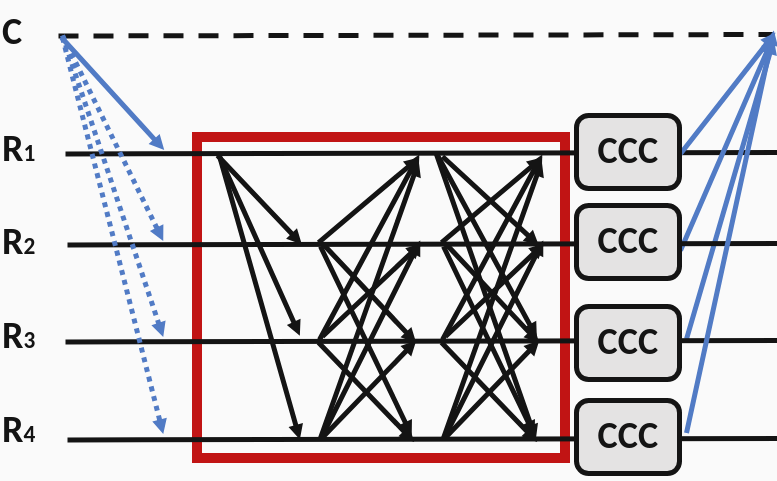
\includegraphics[width= 0.4\textwidth]{./figures/AB.png}
\end{center}
\caption{Atomic Broadcast}
\label{fig:Figure1}
\end{figure}


\begin{figure}
\begin{center}
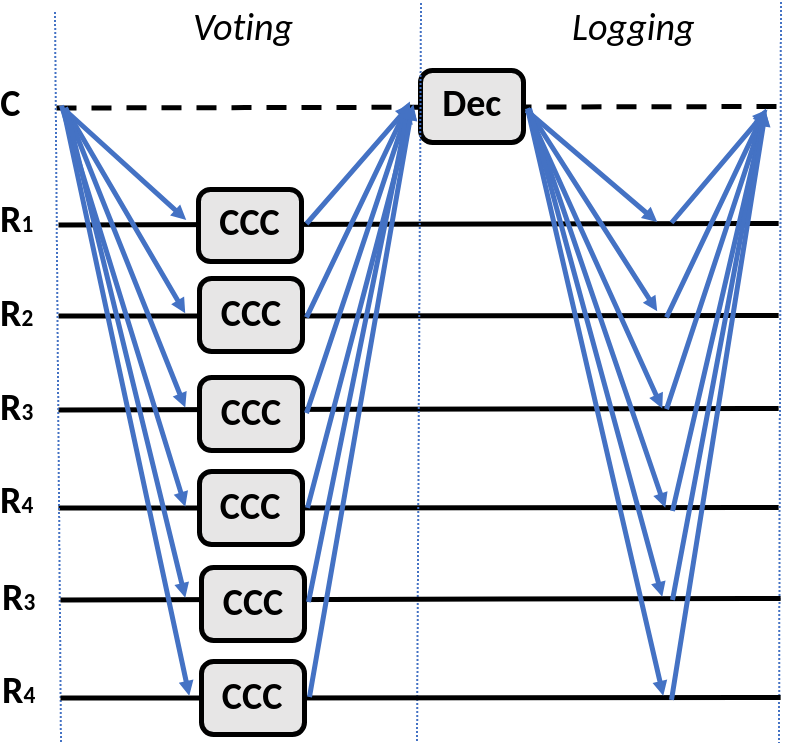
\includegraphics[width= 0.4\textwidth]{./figures/5f+1.png}
\end{center}
\caption{Logging}
\label{fig:Figure1}
\end{figure}

Principles and challenges

protocol overview: pic
\fi

%-------------------------------------------------------------------------------
\subsection{Writeback and Multi-shard 2pc}
%-------------------------------------------------------------------------------

Validation occurs on every Shard that a transaction spans. The goal of the Writeback phase is to aggregate all relevant shard-decisions and to inform replicas of finalized Commit or Abort decisions. This is necessary in order for replicas to be able to garbage collect meta-data of ongoing transactions, and to allow consecutive transactions to reliably observe the updated state. Any finalized decision must respect all shard-decisions relevant to a transaction. Thus, all decisions are aggregated according to standard two-phase commit. Only if all shards agree that a transaction may commit (i.e. there exist commit certificates for every shard), then a transaction may commit. The protocol is simple:

\textbf{1. A coordinator waits for all shard decisions, including certificates}\\
\textbf{2. The coordinator broadcasts a $Writeback \coloneqq (TX, decision, \{certificates_S \} )$ message to all replicas in all relevant shards}.\\

\fbox{
\begin{minipage}{21em}
\textbf{(1 : Coord $\rightarrow$ S)}: A coordinator aggregates decisions and forwards them to all relevant shards.
\end{minipage}
}

A coordinator waits for all shard decisions, including certificates. The coordinator aggregates the decisions and broadcasts a $Writeback \coloneqq (TX, decision, \{certificates_S \} )$ message to all replicas in all relevant shards.
\underline{Additional subtlelties:} A transaction includes a set \textit{InvolvedShards} of relevant shards . A \textit{Writeback} message is only valid if there exists a shard-certificate for every involved shard. The Writeback message does not need to be signed. A single Abort certificate may short-circuit the coordinator wait as it suffices to Abort.\\





\fbox{\begin{minipage}{21em}
\textbf{(2 :  S)}: Replicas in a shard validate and finalize the writeback decision.
\end{minipage}}
Upon reception of a \textit{Writeback} messgage, a replica validates whether a) there exist a single Abort shard-certificate, or b) Commit shard-certificates for all involved shards, and whether its own shard is involved. If not, a replica rejects the request. If the request is valid a replica does the following:\\

\textbf{Abort:} A replica removes the transaction from its OngoingTX set and PreparedDB, and adds the transaction, along with the shard-certificates to its AbortLog. Furthermore, if a set of dependents existed in the WaitingDeps set, the replica resumes the blocked MVTSO checks for the dependents and votes Abort. It clears the WaitingDeps set and all corresponding Dep[dependent] entries in the Deps set.
\fs{this abort log somehow needs to be able to be garbage collected. abort certs are necessary to prove a dependency abort is legitimate - could be replaced by voting abstain}\\


\textbf{Commit:}
Analogous to Abort, a replica updates OngoingTX set and Prepared DB, but adds the transaction, along with certficates to the CommitLog. It additionally updates the key-value Database by creating entries for each read and write. \fs{optional notifiy for early abort:} Furthermore, for all write keys, it removes all existing Read Timestamps (RTS) that are smaller than the committed TXs Timestamp and notifies the clients that issued them. \fs{this allows those clients to abort and restart execution early - requires the commit proof to be accepted by clients}. 
Lastly, if a set of dependents existed in the WaitingDeps set, the replica updates the respective dependencies set for all dependents in Deps (i.e. $Deps[dependent] \setminus TX$). If for any dependent $Deps[dependent] = \emptyset$ then the replica resumes the blocked MVTSO check for the dependent.



\underline{Additional subtlelties:} A byzantine clients transaction might include reads and writes for a shard, yet not include the shard in the \textit{InvolvedShards} set. This is consistent with the definition of Byzantine-Atomicity. Moreover, a replica would have never processed a Prepare message if InvolvedShards does not include its ownShard, and hence no garbage collection is necessary.\\

We point out, that the Writeback coordinator need not be the client issuing the transaction, but can in fact be an arbitrary party (client or replica) that is interested in completing the Writeback. This follows straightforwardly from Theorem Y: Any certified shard-decision implies the existence of a logged decision, and hence the Writeback phase is idempotent.
We utilize this to drive the recovery protocol outlined in section X. 



%-------------------------------------------------------------------------------
\subsection{Granting Liveness}
%-------------------------------------------------------------------------------
\fs{This needs to come out more clearly: shard decision implies logged decision, but there may not be any shard decision. We want logged decision to imply that any honest client can generate a shard-decision. There may neither exist a logged decision, nor enough replicas voting for a shard-decision.
}
Indicus operates under the premise that clients experience progress indepentently. Since agreement occurs on a per Transaction basis (each client drives its own validation) and replicas may process requests out of order, there exists no shared notion of system progress. When all participants are honest progress is trivially guaranteed for every client. Byzantine clients however, may bring execution, validation or writeback to a halt for their own transactions. For example, a byzantine client may either stall during all phases, or equivocate during validation logging. The latter case lets replicas diverge on the decision value (Commit/Abort), making impossible to arrive at a shard-decision, and hence degenerates to a form of stalling too. When all transactions are commutative this phenomenon requires no action: Any client \textit{chooses} whether to adhere to the protocol and experience progress, or not. However, when this is not the case, and transactions depend on each other, either explicitly (through reading anothers transactions uncommitted write), or implicitly (through read-write conflicts), liveness is no longer independent. For instance, a claimed dependency might be of byzantine origin (explicit dependency) and never terminate, causing the dependent to stall helplessly itself. Alternatively, an uncommited write, yet unclaimed dependency, (implicit dependency) might forever cause all consecutive read transactions to abort  \fs{since we only return the max uncommitted as prepare it might not be possible to get enough matching..}.
Thus, in order to allow clients to intertwine their fate with concurrent transactions, we must strengthen Theorem X. We define Liv:

\begin{theorem} \fs{rename to liveness}
For any transaction, there exists \textbf{exactly one} logged decision, if desired by an honest client.
\fs{Any request that an honest client is interested in (broader than just "issued by an honest client") eventually completes}
\end{theorem}
Intuitively, this property would allow honest clients to experience progress, if they desired. To achieve this, we must relax the requirement that replicas may never their decision, while preserving Theorem X (rename to Safety).


A naive solution would be to allow any client to drive another clients protocol. This is problematic, since \textit{interested} clients could concurrently make inconsistent decisions and consequently never make progress. Electing a single client is similarily not live, as there is an unbounded number of byzantine clients that will constructively aid in reconciliation. We circumvent this, by letting concurrent clients replay the protcol, but partially delegating responsibility to the replicas. Concretely, we design a mechanism to elect \fs{endorse ;)} a dedicated \textit{Fallback} replica that is responsible for reconciling diverged replica decisions. Since the number of faulty replicas is bounded, at most $f+1$ leader elections are necessary to make progress when the network is synchronous. A challenge in doing is to guarantee a live round-robin election. We remark, that in an asynchronous network, leader election might not be possible \fs{this is in accordance with FLP, as no non-randomized protocol can reach agreement in an async setting}. \fs{ Contrary to traditional BFT protocols, system progress is a client local property and we strengthen the liveness condition: We can provide liveness only if the system is synchronous and the client is honest}

On a high level, the recovery mechanism operates as follows: \textit{Interested} clients attempt to run the validation protocol themselves. If a client notices or suspects previously present decision divergence, it issues a \textit{Fallback invocation}, i.e. a request to elect a \textit{Fallback} replica to seize control and reconcile decisions. Such recovery protocol is reminiscent of \textit{view-changes} in traditional BFT SMR protocols, but differs in two core aspects: a) While control changes between fallback replicas (leaders), the protocol is still fully client driven (there are no \textit{view-changes} without client invocation) \fs{client does p1, p2, invocation, writeback}, and b) The fallback mechanism impacts only the ongoing transaction, concurrent transactions keep progressing indepentently.

Below, we detail the protocol by following a transactions life cycle. To start the protocol we assume an \textit{interested} client is in possession of the respective transactions $Prepare$ message, signed by the orignial issuer. \fs{this info can be obtained as part of MVTSO check (f+1 must have the TXID, so an honest replica will have the full TX) for own Tx or through an abort (>f+1 abstains necessary, one honest one will return the conflicting reason - subtlelty: there may be multiple different conflicts but only one is returned; it limits how clients become interested. client learns about full PrepareTX in MVTSO check: returned to it for all TX that have not completed yet. This avoids unecessary info in the exec phase (i.e. reads including full TX)}. For sake of exposition we moreover assume that the transaction has not finalized via Writeback on any replica. We briefly discuss this case afterwards.




\fbox{\begin{minipage}{21em}
\textbf{(1: C $\rightarrow$ R)}: Client submits backup Prepare request to all Replicas in all relevant shards.
\end{minipage}}
An interested client broadcast a message $Rec-Phase1 \coloneqq (TX.Phase1, CID)$ to all replicas in \textit{InvolvedShards} of the transaction. 

\fbox{\begin{minipage}{21em}
\textbf{(2: R $\rightarrow$ C)}: Replica receives and processes Client request.
\end{minipage}}
If a replica has not previously processed the same Phase1 message, it executes the normal validation protocol and returns the according reply to both the interested client and orignial client. It furthermore starts a time-out on the transaction and adds CID to a list of \textit{InterestedClients} for the respective transaction.
Otherwise, it skips re-execution and does the following: It adds CID to the list of \textit{InterestedClients} and replies with the transactions state stored in $OngoingTX[TxID]$. This state includes the existing $Phase1R$ reply message and, if existing, a decision value ($Phase2R$ message), as well as the \textit{view.no} of the decision. It additionally includes its current $view$.

\underline{Additional subtlelties}: A replica does not need to return $Phase1R$ if it has a decision. The $view.no$ of the original client is zero. Larger views indicate decisions made by a Fallback replica, specifically by the replica with $RID = view.no \% n$. The current view indicates which is the last $Fallback$ replica a client has attempted to elect (Zero, if none yet). Further, a replica delays the timer start until the transaction has no dependencies of its own. This avoids early client evicition and Fallback election in case progress was justifiably inhibited. \fs{re-iterate this to be in sync with mvtso check. Where to block; one could argue the Timestamp is not started because it is still waiting. Hence no replies are issued either.}

%%Fallback start
\fbox{\begin{minipage}{21em}
\textbf{(3: C $\rightarrow$ R)}: Client receives responses and either returns to Writeback or invokes \textit{Fallback} election.
\end{minipage}}

We distinguish the following two cases:

\fbox{\begin{minipage}{21em}
\textbf{(3a: C $\rightarrow$ R)}: A client receives the necessary information to proceed to Writeback.
\end{minipage}}
We consider two subcases:\\
a) If a client receives enough matching $Phase1R$ messages to fulfill a Fast-Path Threshold, it can move on to Writeback. This is safe, because these are logged decisions and imply that any potenially existing Slow-Path decision is the same.
b) Alternatively, if a client receives enough matching (in decision and view) $Phase2R$ messages to form a certificate it proceeds to the Writeback phase.\\


\fbox{\begin{minipage}{21em}
\textbf{(3b: C $\rightarrow$ R)}: A client needs to go Slow-Path or observes inconsistency and requires assistance for resolution.
\end{minipage}}

If a client receives $\geq f+1$ matching decision values and views ($Phase2R$ messages; favors Commit if two matching sets exist) it forwards those to the replicas as proof for a new $Phase2$ message (with the same decision) that it broadcasts to all replicas. If it instead receives $< f+1$ matching decisions it uses the received $Phase1R$ messages to iniate its own $Phase2$ message (identical to validation step, but signed by this client). 
Additionally, if the client received inconsistent decisions (i.e. both Commit and Abort) or $<f+1$ total decision messages that differ from its own proposed decision, it initiates a \textit{Fallback election}. To do so, it broadcasts a message $electFB \coloneqq (TxID, CID, \{view\}_R$. It attaches a set of $4f+1$ signed view messages.  

\fs{refine this}
\underline{Additonal subtlelties}: A client may treat a $Phase2R$ decision as $Phase1R$ vote for the sake of making a new decision. This is safe: If the replica was honest, then this reflects that there existed enough matching votes, and if it was byzantine, it could have voted arbitrarily regardless. \fs{maybe just simpler if replicas include their phase1r as well, but this adds overhead}
 \textbf{View Change Rules:} A client sends a set of signed view messages in order to let potenially diverged replicas now what next view to vote for. However, replicas only adopt a view $v+1$ if the view set includes $3f+1$ \fs{3f+1 should be enough: satisfies that f+1 votes will be found. Can use 4f+1 instead otherwise} votes from view $v$. \textit{Vote subsumtion:} A view $v$ subsumes all prior views: I.e. a replica vote $v$ may count as a vote for all $v' \leq v$. If a byzantine client attempted to diverge the views by only invoking a view change for a subset of replicas, such matching set of views might not exist. 
Replicas that lag behind, may catch up to the maximum view $v$ present $f+1$ times. Such view vote implies, that at least one honest replica has voted for view $v$, and would have done so only, if $2f+1$ honest replicas had previously been in view $v-1$. The possible divergence can be reconciled in a single step, since there must always exist some view $v'$ for which at least $f+1$ honest votes exist in any Quorum (set of 4f+1 voteS) such that $v' \geq max(honest.views) -1 $ (see Vote subsumtion). Thus, the next view change incurs at most 1 additional Roundtrip, since all honest replicas either join max(honest.view) (no additional overhead) or max(honest.view)-1 (another roundtrip to gather $3f+1$ votes.)



\fbox{\begin{minipage}{21em}
\textbf{(4: R $\rightarrow$ C)}:  Replicas receive $Phase2$ messages 
\end{minipage}}
We break the procedure into two components:

\fbox{\begin{minipage}{21em}
\textbf{(4a: R $\rightarrow$ C)}:  Replicas replies with decision
\end{minipage}}
If a replica receives a valid $Phase2$ request (see Validation) it adopts the decision and replies with a corresponding $Phase2R$ message.

\underline{Additional subtlelties:} A replica will buffer requests from $CID \neq originalCID$ and process them only \textbf{after} the timer (set in step 2) expires. If the client request includes a proof of inconsistency (see step 3 and 4b) it will ignore the timer and process the request immediately. If a replica previously adopted a decision, it treats the new request as no-op and returns the stored decision.


\fbox{\begin{minipage}{21em}
\textbf{(4b: R $\rightarrow$ R(FB))}:  Replica additionally receives Fallback invocation and starts election
\end{minipage}}

If a replica receives an $electFB$ message and the original client has timed-out it attempts to elect a new \textit{Fallback replica}. To do so, it follows the \textbf{View Change Rules} and adopts new view $current.view = v$ if $v > current.view$. \fs{effectively when a replica adopts a view, it ignores all older views. Trivial, since it only accepts the first p2 and then never changes. Only thing that changes this is a FB message from higher view.}
Replicas send an $Elect \coloneqq (TxID, decision, current.view)_R$ to replica $current.view + TxID \% n$.


\underline{Additional subtlelties:} 
When byzantine clients attempt to invoke elections they may only send the request to a subset of honest replicas, thus never truly enabling an election (requires $4f+1$ elect votes). If there are no concurrent honest interested clients, this can result in replicas being skipped in consideration to become the next Fallback. Moreover, to achieve liveness, we assume a weakly synchronous model, and hence increase the timeouts for each view exponentially.
In order to avoid artificially increased timeouts and enforce a round robin election without skipped candidates, replicas can forward the $Elect$ message to all other replicas. If another replica receives $f+1$ such messages, it adopts the view and sends an $Elect$ message of its own. This ensures, that for each view, a Fallback is indeed elected (if the network is synchronous within timeout $\delta$). This optimization only aids practical progress in the face of misbehavior and is not necessary for theoretical liveness. To avoid unecessary all-to-all communication, it may only be enforced for views $v > T$, where T is some system defined threshold. \fs{We choose T = f, to avoid false client suspicion in case the first f Fallbacks were byzantine and never replied} 



\fbox{\begin{minipage}{21em}
\textbf{(5: R(FB) $\rightarrow$ R)}:  Fallback aggregates and echos election messages.
\end{minipage}}
The Fallback replica considers itself elected upon receiving a Quorum of $4f+1$ Elect messages. It then uses this set of messages to reconcile a decision. It broadcasts a message $FBdec \coloneqq \langle RID, dec, view, \{Elect_r\} \rangle_R$, including the new decision and the Elect messages as proof. Effectively, replicas compute the new decision themselves; the Fallback acts as single broadcast channel in order to guarantee that all replicas receive the same Quorum of states.

\underline{Additional subtlelties:} A byzantine Fallback may equivocate Elect Quorums. However, after at most $f+1$ fallback elections a consistent result will be derived (given Synchrony).
\textbf{Decision Reconciliation Rule:} The reconciliation rule is straightforward: $dec_{new} = majority(\{Elect.decision\})$. If a logged decision exists (implies that a shard-decision might exist), any Quorum of $4f+1$ Elect messages is guaranteed to contain $2f+1$ matching decisions (a majority). Vice versa, if $<2f+1$ replicas agree on a decision, then it is impossible for this decision to have been logged. Thus it is guaranteed that logged decisions persists and otherwise an arbitrary decision qualifies since at least one honest replica must have proposed it (and hence the decision is based on a legal $Phase2$ Quorum).
\fs{optional: If a Fallback receives $>4f+1$ Elect messages, he may choose a Quorum that favors Commit (maximizes dependencies commit chance, but gives byz clients benefit of the doubt).}



\fbox{\begin{minipage}{21em}
\textbf{(6: R $\rightarrow$ C)}:  Replicas echo decision to interested clients
\end{minipage}}
Replicas receive a $FBdec$ message and validate the legitimacy of the Fallback replica as well as the new decision. If $FBdec.view \geq current.view$ it then updates its decision and decision view, $decision = (FBdec.dec, FBdec.view)$ and sends a $FBcomp \coloneqq \langle(Phase2R, current.view\rangle_R$ message with the respective decision to all interested clients.

\underline{Additional subtlelties:} If replicas time-out waiting for a $FBdec$ message, they forward their current view to all interested clients. If $FBdec.view > current.view$ it updates its current view as well.

\fbox{\begin{minipage}{21em}
\textbf{(7: C}: A client starts Writeback phase or restarts Fallback invocation
\end{minipage}}
An interested client waits for $\geq 4f+1$ $Phase2R$ replies up to a time-out. If it received enough \textit{matching} decisions to form a shard-certificate it proceeds to the Writeback phase. If it times out, receives insufficient, or inconsistent decisions it re-starts Fallback election by broadcasting $electFB \coloneqq (TxID, CID, \{view\}_R$, for the new set of views received.

\underline{Additional subtlelties:} Only matching decisions from the same view qualify as shard-certificate. The attentive reader may notice that Elect messages however do not include the view in which a decision was made. These need not be from matching views as follows straightforward via Induction: If there ever existed a shard-certificate, then there existed a logged decision $d$ with matching views. Thus, by the Decision Reconciliation Rule, all future $dec_{new} = d$ and hence it is safe to rely on decisions from different views (- it is in fact necessary, as the Fallback may be byzantine and not broadcast to all replicas).
A client \textit{expects} to receive $4f+1$ matching decisions and will continue to wait for decisions from the same view if the first $4f+1$ messages received match in $\geq 3f+1$ cases. Upon time-out, a client proactively starts a new election (keeps waiting regardless) in case the past \textit{Fallback} was byzantine or did not succeed in timely reconciliation. Eventually a logged decision must exist and time-outs grow enough to guarantee a client will receive $4f+1$ matching. In section X (optimization) we discuss a practical optimization.
 \\


%%%%%%%
Any honest client that follows the Fallback protocol experiences \textit{Liv}. This follows straightforward from the eventual existance of an honest Fallback replica that reconciles all honest replicas. Thus, if an honest client is interested, a decision will be logged and eventually a shard-certificate will be received.

We want to point out that steps 1, 2a, 3 and 4a simply correspond to the normal validation protocol. Such execution might be necessary in case the original client suffered from omission (potentially byzantine) or was simply slow (i.e. there are no inconsistencies). In order to avoid \textit{interested} concurrent and/or byzantine clients claiming power too soon and causing unecessary divergence, we grant the original client an initial window of immunity.
However, after this timer expires this transaction becomes "fair game" and anybody client can claim responsibility on termination. The orignial client too, is an interested client by default - an honest client that loses autonomy will still attempt to complete the protocol, and, if necessary elect a \textit{Fallback} itself. If the original client is byzantine, yet no other client is ever interested, a replica may eventually turn into an interested "client" itself in order to drive forward garbage collection.
Note, that it is irrelevant which client issues the $Phase1$ message. Furthermore, it is both safe and "fair" for any client to return to the Writeback phase using a Fast Path. Therefore, we enforce the timeout window only for explicit logging ($Phase2$). 

When depending on slow or byzantine transactions, clients may have to incur extra latency in order to maintain liveness. \fs{Overall, if FB invocation necessary and worst case: 1 rr voting, 3 rr FB (+1 wb) for dependencies (can be in parallel for all), 1 rr logging + 1 rr own wb.}
This is the price they pay in order to experience liveness independently from the rest of the system. On the flipside, when a clients fate is independent from other transactions, it is entirely unaffected by concurrent "view-changes". Clients that are caught equivocating or responsible for for frequent time-outs may be excluded from the system. In order to participate in a consortium database meeting performance standards is a requirement.

\fs{Fallback replicas that equivocate can be expelled. Clients that equivocate cannot be expelled because one potentially cannot tell the difference between concurrent and single client. Instead, they can get punished for being slow.}

%%%%%%%%%%%%%%%%%%%%%%%%%%%%%%%%%%%% WRITEBACK HAS ALREADY HAPPENED
\textbf{Finalized decisions:} If a replica has already received a Writeback message for a transaction it ignores all Fallback related client requests and simply returns the Writeback decision, and additionally the Writeback certificate if not yet garbage collected. A client may use either this certificate or $\geq f+1$ matching decisions to issue the Writeback for other replicas. In the following section we discuss how to perform certificate garbage collection in a manner that maintains liveness.

%-------------------------------------------------------------------------------
\subsection{Garbage Collection}
%-------------------------------------------------------------------------------
In section X (Writeback) we previously discussed how replicas garbage collect finalized \textit{Ongoing Transaction State}. We now briefly allude to garbage collecting unecessary certificates as well as outdated versions.

\textbf{Certificates}: Honest replicas store decision certificates for two purposes: a) It allows them to singlehandedly propagate Writeback decisions and b) It allows Validation to return on Abort Fast Paths by providing conflict proofs. In theory, certificates may be removed whenever, as storing them is not necessary for correctness (the existance of a certificate implies the existance of a logged decision). Replicas must then vote to Abstain where they previously voted to Abort (we point out that the existance of a logged decision implies that voting Abstain instead of Abort is always safe). Since certificates are comprised of signature Quorums they impose costly storage overhead and are hence important to garbage collect swiftly.
However, in order to guarantee that garbage collection is \textit{final}, i.e. no state is re-opened, we need to stricten the requirement on when to remove obsolete certificates. Concretely, we must confirm that enough replicas have finalized the decision, in order to guarantee that every interested client receives $\geq f+1$ matching decisions. \fs{Otherwise, a client might receive too few p2 decisions in order to start fallback, because finalized replicas ignore requests. In this case replicas would have to "play along" and let their decision be treated as p2. This requires re-opening Ongoing TX state, that may never be closed if there is no interested honest client} To facilitate this, we add an additional client-replica exchange off the critical path:

\fbox{\begin{minipage}{21em}
\textbf{(2: R $\rightarrow$ C)}:  Replicas receive and acknowledge Writeback decision
\end{minipage}}
Upon receiving and processing a valid Writeback decision a replica returns an acknowledgement message $EchoWB \coloneqq \langle TxID, decision \rangle_R$.

\fbox{\begin{minipage}{21em}
\textbf{(3: C $\rightarrow$ R)}:  Client aggregates acknowledgements and forwards them
\end{minipage}}
The client waits for $2f+1$ matching decisions, bundles them, and forwards them to all replicas.

\fbox{\begin{minipage}{21em}
\textbf{(4: R ($\rightarrow$ R))}:  Replica receives garbage collection confirmation
\end{minipage}}
Upon receiving $2f+1$ discrete replica confirmations a replica is aware that $\geq f+1$ honest replicas have finalized the decision and hence will assist any honest client in re-issuing the Writeback phase.

\underline{Additional subtlelties:} If a replica does not receive client acknowledgements within a time-out (a low Watermark for garbage collection has been reached), it broadcasts the $EchoWB$ message to all replicas. \fs{alternatively only forward to 3f+1 in a round robin scheme, GC as soon as $2f+1$ received}


Next, we discuss how to prune old versions from the store.



\textbf{Versions}: We keep a shared \textit{low Watermark} that denotes what versions can be pruned. Whenever \fs{it is also fine to do it less frequent} a write (on any key) occurs, we advance the Watermark to $lowWM = localClock - \delta$. We then prune all versions $< lowWM$, the latest version being exempt in order to maintain at least one version. \fs{periodically, we may do this for all keys in order to also prune "inactive" keys that still have multiple versions.} We point out, that client reads with $TS < lowWM$ may fail once we prune the genesis version. This does not imply transaction abort, since clients are free to change their timestamp and retry a read during execution.
\fs{we might want to abstain from transactions even if we did not prune the log, because those do not offer efficient lookups for conflicts: I.e. move the abstain logic for TX to this paragraph, and only keep dependency abstains in the log section.}

\fs{Read versions below watermark: must abstain because it is unknown whether conflicting writes were already garbage collected. Write TS below watermark: must abstain because it is unknown whether conlicting reads were gc.}
\textbf{Log Entries}: We store all committed or aborted transactions in respective Commit/Abort logs. These are un-ordered sets and allow both for fast lookup during Validation as well as offline audit off all transactions. For example, an audit on transaction reads or writes may be performed in order hold byzantine clients responsible for participation in the system. Illegal reads or non-atomic writes can be discovered and serve as Proof of Misbheavior to expell a client. When audit is not desired, we can garbage collect old transaction decisions. We can remove CommitLog entries whenver a respective version of one of its writes (i.e. the first or last) is pruned. AbortLog entries instead can be removed whenever the Low Watermark increases (need not happen on every update, but periodically). 
In order to maintain Isolation, a replica must vote to Abstain from every new transaction with timestamp below the low watermark. Such a transactions reads and writes cannot be checked for conflicts anymore, as existing conflicts might have been garbage collected already. \fs{for reads: we can be a little more fine-grained: If there still exists a version that is smaller than the low WM, then no gc has happened yet and isolation is still safe. For writes this is not the case: cannot know whether there was a read above the write TS but below the WM that has been gc. } Additionally (for the same reason), replicas must Abstain from transactions that read versions below the watermark.
Lastly, replicas must abstain from any transaction that has a dependency with $dep.version  < lowWM$ \fs{dep version is the timestamp of such tx}, as its dependency could have been garbage collected already. \fs{in this case it would block infinitely. We can be a little more frine-grained: only need to abstain if the dep is not in the commit log. If it is, there is no need to abstain}. 






%-------------------------------------------------------------------------------
\subsection{Optional Modifications}
%-------------------------------------------------------------------------------
Next, we discuss a series of optional optimizations: \fs{not necessarily optimizations: Retries, Single shard logging, speeding up shard certificates, read leases}

\fs{retries come at the cost of no fast path and having to store proofs for the transaction. These proofs are only necessary for the fallback.}
\fs{If limiting Fallback}
\textbf{Retries:} MVTSO, by design, favors read requests, at the cost of potentially aborting concurrent write transactions. This is intuitively sensible, as reads require additional WAN roundtrips in order to execute. 
However, when a transaction includes both reads and writes, and execution spans several reads, it becomes increasingly suceptible to abort as consequence of a conflicting read request. Observe, that aborts due a write-read conflict are a consequence of a read having failed to observe a relevant write with smaller timestamp. Thus, such an abort could have been avoided by simply choosing a larger timestamp. In order to faciliate this, we offer write transactions the option to Retry (with a larger timestamp), rather than abort. This however, comes at a tradeoff: Clients may not utilize the validation Fast-Path when opting into the availability of Retries. We outline the Retry protocol and implication for Fast-Paths as follows:

In order to be able to change the timestamp for the same transaction we must make the Transaction ID independent from it. Thus, we re-define $TxID \coloneqq H(TX \setminus TS)$. A Prepare message then takes the form $Phase1 \coloneqq \langle Prepare, TxID, TX, TS \rangle_{\sigma c}$
Effectively, timestamps act as \textit{Retry Heights}: Analogous to views, only retries from a larger height can superseed previous attempts. Only the original client may retry, up to a pre-defined maximum attempts.


- replicas keep p1s for all heights; might be necessary in case it still commits (for both safety and liveness: need to maintain isolation, need to reply with enough p1s.)
Never accept more than 1 p2, othwerise it could be committed twice.

- replicas dont accept retry prepare if they have received a p2. (might need to not do this, in order to create enough p2s for the fallback?)
- dont accept p2 from smaller height if larger p1 has been accepted. (might need to not do this, could be difficult to find the correct height)
- if a byz client equivocates p2 with different timestamps we must reconcile this in the recovery protocol. 

- cant allow fast path: then a TxId could commit/abort fast path but commit/abort slow path with 2 different timestamps. If we made the timestamp part of the ID. then we couldnt track that it is the same TX. garbage collection would be impossible and we might lose state necessary for safety.

Require proofs of p1s in the p2 decisions: because we might not get enough matching p2 ether. need to be able to decide based off just 1.

Fallback (p2 certofocates from 2 different heights cannot co-exist. if the rules for fallback dont fire, i.e. if there is none with >=2f+1 matching: choose larger height that has >=f+1 matching. Else make decision of p1s: (are included in the decision)

Correctness of retries: Show how MVTSO is fine with it. Adds additional check for dependencies TS. 
If a TX retries: Its read locks might have been useless, i.e. doing the CC check might fail now. 
If a dependency retries: If the dependencies writes would now be bigger than own TS then own TX needs to abort upon being released from blocking. I.e. before returning check and change the result to abstain.






- Retries can be per client choice (have a flag in a TX that says whether fast path or retires available). Cannot have both fast path and retries.

\paragraph{Single shard logging}
When transaction execution touches multiple shards validation can incur redundant explicit logging overhead. When a Slow-Path is necessary to arrive at a logged decision on S different shards, bandwith is wasted. Consider an example in which $S-1$ shards attempt to log the decision Commit, while a single shard attempts to log an Abort decision. If the latter shard succeeds, the effort of the remaining shards was in vain. 
The culprit of this phenomenon is the delayal of Two-Phase-Commit (2PC) until the Writeback phase. By preemptively making a 2PC decision \textbf{before} logging we can avoid this redundancy. We remark, that even when when all shards agree on a decision, this saves redundant coordination.
Concretely, we designate \textbf{one} involved shard as \textit{logging Shard}, while all other shards remain responsible only for Validation. Figure \ref{fig:SingleShardOpt} shows the revised structure. In order to log a decision, voting quorums from all involved shards are required. We modify step 3 of the Validation protocol accordingly:

\fbox{\begin{minipage}{21em}
\textbf{Validation (3: C)}: Client waits for vote replies from all involved Shards.
\end{minipage}}
For each involved shard, a client waits for at least $n-f$ ($4f+1$ in Indicus5) distinct replica votes, or more, up to a system specified timeout. A client aggregates a per-shard decision for each shard according to the \textit{CommitQuorum} rule. If all shard-decisions are Commit, it attempts to log a Commit decision by sending $Phase2 \coloneqq (TxID, Commit, S \times \{CommitQuorum\}$ to all replicas in the designated logging Shard. If a single shard-decision is Abort, it stops waiting for other shard-decisions and attempts to log an Abort decision by instead sending $Phase2 \coloneqq (TxID, Abort, AbortQuorum)$. 

\underline{Additional subtlelties:} A client can go Fast-Path and return to the Writeback phase immediately only if Fast-Path Quorums were received for all shards. Logging is always bottlenecked by the slowest shard. The logging Shard can be determined via a determinsitic function over the \textit{involved Shards}. A simple solution can designate the shard with lowest ID. A load balanced function could select $loggingS = min(TxID \% involvedShard)$.

The remaining Validation protocol proceeds identically to the multi-shard version. Notice, that when only a single shard is involved, no adjustments were made. The Writeback phase instead, may proceed with just the single certificate from the logging Shard: 

\fbox{
\begin{minipage}{21em}
\textbf{Writeback (1 : Coord $\rightarrow$ S)}: A coordinator receives certificate and forwards them to all relevant shards.
\end{minipage}
}
A coordinator waits for the logging shard decision, including shard-certificate, and broadcasts a $Writeback \coloneqq (TX, decision, certificate_loggingS )$ message to all replicas in all relevant shards.

The Fallback protocol is adjusted accordingly: A fallback replica need (and can) only be elected on the logging Shard, simplifying reconciliation and reducing the cost for interested clients. 


\begin{figure*}
\begin{center}
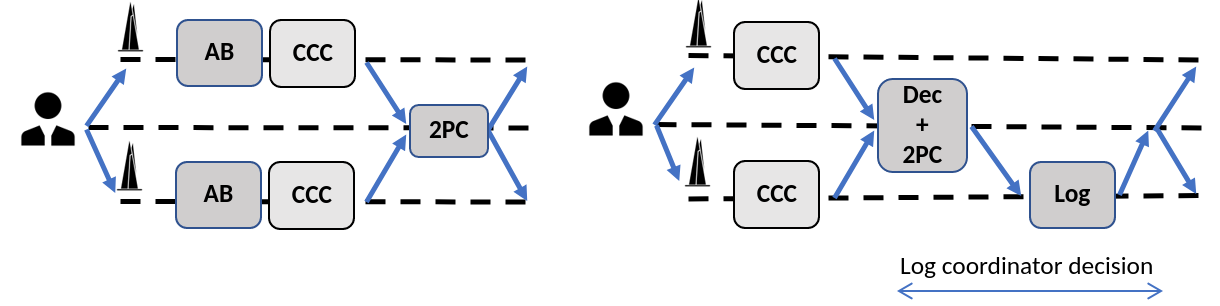
\includegraphics[width= \textwidth]{./figures/SingleShard.png}
\end{center}
\caption{Single Shard Optimization}
\label{fig:SingleShardOpt}
\end{figure*}



\paragraph{Shard decisions}

%%%%%%%%%%%%%%%%%%%%%%%%%%%%%%
\fs{How to get from logged decision to shard certificate: We do not implement this optimization}

When network message delays are not withing synchronous bounds an \textit{interested} client may not receive $4f+1$ matching decisions until time-outs grow large enough. To short-circuit this wait, we can add an aditional, non critical-path, roundtrip in order to achieve liveness when the network is truly asynchronous: \fs{note, that in an asynchronous network a fallback may never be elected and reconciliation might be stuck} 
Concretely, a client may use $3f+1$ matching decisions as proof to issue a $Phase3 ...$ decision message. Replicas echo this decision, and clients may return to the Writeback phase with just $3f+1$ $Phase3R$ messages. In order to maintain safety, the \textit{Decision Reconciliation Rule} must be modified. Replicas additionally report existing $Phase3$ decisions to a Fallback replica. If there exist $f+1$ Phase3 decisions we need to adopt this decision \fs{both as p2 and p3 decision is fine}. This is safe because a) no two Phase3 decisions can co-exist in the same view \fs{since 3f+1 votes must intersect in one honest}, b) the existance of a logged decision implies that any $Phase3$ message must comply with this decision, and c) the existance of a $Phase3$ certificate implies that the decision will be logged. \fs{decisions go by view precedence: phase 2 from higher view counts over phase 3 from lower view. These can be inconsistent if the decision was not logged and a p3 is generated, a view change happens without the p3 messages, and now the p3 are different from p2. But those p3 could not have been returned, otherwise f+1 would have been included in view change. Replicas dont send p3 for smaller view once new view is adopted.}
We remark, that this optimization does \textbf{not} imply that a client must wait for three roundtrips to complete, but rather may use the $Phase3R$ decisions if waiting on remaining $Phase2R$ decisions turns out to be slower.

\iffalse
\textbf{Finalized Fallbacks}
Fallback finish certificates (and do writeback themselves).\\
%%%%%%optional
\fbox{\begin{minipage}{21em}
\textbf{(6: R $\rightarrow$  FB)}:  Replicas echo decision to Fallback
\end{minipage}}


\fbox{\begin{minipage}{21em}
\textbf{(7b: FB $\rightarrow$ R)}:  FB sends p3 as final certificates. Can be writeback if only single shard involved, or if replicas know about all other shards.
\end{minipage}}



\fbox{\begin{minipage}{21em}
\textbf{(8: R }:  store certificate. use it to reply to clients that ask in the future if necessary.
\end{minipage}}
%%%%%%%%%%%%%%%%%%%%%%%%%%%%%%%%%5
\fs{END}
\fi



\textbf{read leases}: only for a time (does not matter so much; concurrent tx should get past that TS anyways). But if a client has a history of expired leases, then grant no more, or grant shorter and shorter.
- (Read Locks ; remove can be optimization for writes)

 Read leases instead of unlimited locks - in practice only grant to timely clients (not a safety measure, but an increased progress guarantee)

- OCC instead of mvtso structures if disallowing prepared writes to be visible. OCC if not worried about reads aborting



\textbf{Reduce tx object content per shard.}
\fs{Each shard should only store the objects necessary for its shard: changes ID.
keep track of not just involved shards, but of involved sub TXIDS: Each shard involved has a different TXID: Each sub TX object includes a list of the other TXIDS. An honest client experiences atomicity by bundling - doesnt work straightforward because cyclic. Need 2 levels of ID.}

\paragraph{Optimization}: 


Optimization:
- validation effort redundant, select single shard to do it


%-------------------------------------------------------------------------------
\subsection{Indicus3}
%-------------------------------------------------------------------------------
3f+1 if not defending against byz colluders as much

- no fast path
- Commits in 2 rounds, Aborts in 3 (Alternatively symmetric version)
- fallback quorums and bounds
- proofs necessary for recovery
- recovery rules

\iffalse
\begin{figure}
\begin{center}
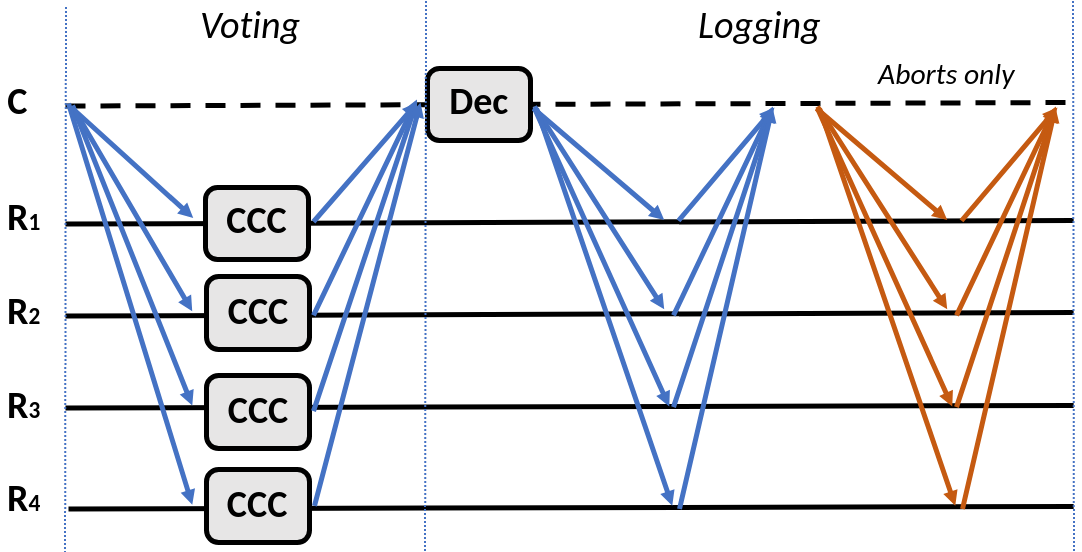
\includegraphics[width= 0.4\textwidth]{./figures/3f+1.png}
\end{center}
\caption{Logging}
\label{fig:Figure1}
\end{figure}
\fi

